\documentclass[12pt,oneside,a4paper]{amsbook} % yksipuoleinen tulostus
%\documentclass[12pt,twoside,a4paper]{amsbook} % kaksipuoleinen tulostus
%\usepackage[leqno]{amsmath}
%\usepackage{amsthm}
\usepackage{amssymb}
%
\setlength{\textheight}{9in} % amsbook default: 632pt
\setlength{\textwidth}{6in}  % amsbook default: 360pt
\setlength{\topmargin}{0in}
\setlength{\oddsidemargin}{0.4cm}
\setlength{\evensidemargin}{0.4cm}
%
\usepackage[T1]{fontenc}
\usepackage{ae}
\usepackage{bbm}
\usepackage[english,finnish]{babel}
\usepackage[dvipsnames]{xcolor}
\usepackage{transparent}
\usepackage[colorlinks,linkcolor=blue,citecolor=blue,urlcolor=blue,bookmarks=false,hypertexnames=true]{hyperref} 

%% Input encoding: valitse tekstieditorisi käyttämä
%% vaihda my\"os dokumentin ensimmäinen rivi vastaavasti
%\usepackage[utf8]{inputenc}           % !TeX encoding = utf8
%\usepackage[latin1]{inputenc}        % !TeX encoding = latin1
%\usepackage[applemac]{inputenc}    % !TeX encoding = appleroman
%
%\usepackage[dvips]{graphicx}
%\usepackage[pdftex]{graphicx}
\usepackage{graphicx}

\usepackage{subfiles}

\graphicspath{graphics}

\renewcommand\thesection{\arabic{chapter}.\arabic{section}}
\renewcommand\thesubsection{\arabic{chapter}.\arabic{section}.\arabic{subsection}}
\renewcommand\thesubsubsection{\arabic{chapter}.\arabic{section}.\arabic{subsection}.\arabic{subsubsection}}
%
%% AMS-LaTeX -määrityksiä
%
\theoremstyle{plain}
\newtheorem{theorem}{Lause}[chapter]
\newtheorem{lemma}[theorem]{Lemma}
\newtheorem{corollary}[theorem]{Seuraus}
%
\theoremstyle{definition}
\newtheorem{definition}[theorem]{Määritelmä}
\newtheorem{example}[theorem]{Esimerkki}
%
\theoremstyle{remark}
\newtheorem{remark}[theorem]{Huomautus}
%
\numberwithin{equation}{chapter}
\numberwithin{figure}{chapter}
%
%% Uusia komentoja, macroja
%

\newcommand{\R}{\mathbb{R}}
\newcommand{\Rp}{{\mathbb{R}^{+}}}
\newcommand{\N}{\mathbb{N}}
\newcommand{\E}{\mathcal{E}}
\newcommand{\dt}{\text{d}t}
\newcommand{\Borel}{\mathcal{B}}
\newcommand{\indfct}[1]{\mathbbm{1}_{#1}}

\newcommand{\what}[1]{\colorbox{red}{#1}}                        % Selvitä, mitä tarkoittaa tai miksi näin.
\newcommand{\whytho}[1]{\colorbox{orange}{#1}}                   % Perusteltava tarkemmin.
\newcommand{\todo}[1]{\colorbox{SkyBlue}{\textbf{TODO: #1}}}    % Tee myöhemmin tähän.
\newcommand{\define}[1]{\colorbox{YellowGreen}{#1}}              % Käsitteen määritelmä puuttuu.

\DeclareMathOperator*{\esssup}{ess\, sup}
\DeclareMathOperator{\supp}{supp}
%
%% Uusia komentoja, päällekirjoitetut
%
\renewcommand{\P}{\mathbf{P}}
\renewcommand{\d}{\text{d}}
\renewcommand{\check}[1]{\colorbox{Lavender}{#1}}              % Varmista, onko oikein.

\begin{document}
\subfile{sections/coverpage} % Kansilehti ja sisällysluettelo coverpagen sisällä
\pagebreak

\chapter{Johdanto}
%
Tämän kirjoitelman tarkoituksena on perehtyä massansiirtoteorian perusteisiin ja erityisesti niin kutsuttuihin liikennesuunnitelmiin.
Ihmiset ovat kautta aikojen ratkoneet ongelmia liittyen tavaran kuljettamiseen paikasta toiseen. Kaupat tarvitsevat tuotteita useista tehtaista. Koko kaupungin kattava vesijohtoverkosto pyrkii kuljettamaan jokaiselle asukkaalle riittävästi vettä. Julkisen liikenteen tehtävä on kuljettaa ihmisiä ympäri maan paikasta toiseen. Kaikille näistä ongelmista on oleellista kustannusten minimointi; tavara tai ihminen halutaan kuljettaa mahdollisimman tehokkaasti. 
Kuvitellaan, että jokin kauppa saa tuotteensa kahdelta tehtaalta. Kaupan tehtävänä on ratkaista, onko esimerkiksi tehokkaampaa tuoda tavara molemmista kaupoista erikseen vai kuljettaa tavara ensin johonkin paikkaan kauppojen ja tehtaiden väliin, josta riittää vain yksi kuljetus kauppaan?

Mielenkiintoista on, että ihmisen suunnittelemat verkostoratkaisut tämän kaltaisiin logistisiin ongelmiin muistuttavat vahvasti luonnossa esiintyviä ratkaisuja samankaltaisiin ongelmiin. Esimerkiksi Suomen tieverkostossa ja ihmisen verisuonistossa voidaan nähdä samankaltaista haarautuvaa systemaattisuutta. Suomen tieverkoston tehtävä on siirtää liikennettä paikasta toiseen siten, että se kattaa mahdollisimman ison asuinalueen, mutta kustannusten minimoimiseksi teitä rakennetaan mahdollisimman vähän. Verisuoniston tehtävänä on siirtää verta sydämestä koko kehoon mahdollisimman vähällä energialla. Molemmat verkostot pyrkivät ratkomaan saman ongelman: miten siirtää massa mahdollisimman vähillä kustannuksilla paikasta toiseen? 

Mallinnetaan esimerkkinä massansiirtoa vesijohtoverkoston näkökulmasta. Oletetaan, että kaikki käytettävät putket ovat suoria ympyrälieriöitä, seinämiltään yhtä paksuja ja niiden sisällä vesi virtaa yhtä nopeasti. Merkitään putken $k$ läpi kulkevan virtauksen tilavuusnopeutta $\phi_k$, putken pituutta $l_k$ ja putken ympärysmittaa $s_k$. Putken $k$ materiaalin kustannus tulee tällöin olemaan suoraan verrannollinen pituuteen $l_k$ ja ympärysmittaan $s_k$ nähden. Toisaalta nähdään, että ympärysmitta on suoraan verrannollinen tilavuusnopeuden neliöjuureen $\phi_k^{1/2}$. Tällöin putkista koostuvan verkon $G$ kokonaiskustannus $C$ voidaan määritellä summana
    $$C(G) = \sum_k l_k \cdot \phi_k^\frac{1}{2},$$
jolloin ongelmana on etsiä verkko, joka minimoi kokonaiskustannuksen.

Massan siirtämisen tutkiminen katsotaan alkaneen Gaspard Mongen (1746-1818) esittämästä ongelmasta \cite{monge} siirtää kasa hiekkaa toiseen paikkaan mahdollisimman vähällä työllä. Moderni, niin kutsuttu Mongen-Kantorovitsin ongelma mallintaa siirrettävää massaa mitoilla. Olkoon annettuna kaksi massajakaumaa $\mu^+$ ja $\mu^-$ avaruudessa $\R^n$, joilla mallinnetaan kysyntä- ja tarjontajakaumia. Siirtosuunnitelmaksi kutsutaan avaruuteen $\R^n \times \R^n$ määriteltyä mittaa $\pi$, jolloin $\pi(A\times B)$ kuvastaa joukosta $A$ siirrettävää massaa joukkoon $B$. Siirtosuunnitelman tehokkuuden laskemiseksi määritellään kustannusfunktio $c:\R^n\times \R^n \to \Rp$, jolloin $c(x, y)$ antaa kustannuksen siirtää massaa pisteestä $x$ pisteeseen $y$. Siirtosuunnitelman kokonaishinnaksi määritellään tällöin $\int_{\R^n\times \R^n} c(x, y) \, d\pi(x, y)$. Mongen-Kantorovitsin ongelmana on tällöin etsiä siirtosuunnitelma $\pi$, joka minimoi kokonaishinnan. \cite[s. 11]{optimal} Mongen-Kantorovitsin ongelman muotoilussa ei kuitenkaan oteta huomioon, kuinka massaa siirretään paikasta toiseen. Muotoilussa voidaan ajatella, että jokainen massahiukkanen siirrettäisiin suoraa reittiä päämääräänsä. Tämä mallinnus ei ole kuitenkaan kovin realistinen, sillä valtaosassa käytännön massansiirto-ongelmista on suotuisampaa käyttää saman massan kuljettamiseen yhtä reittiä, kuin kahta pienemmän kapasiteetin reittiä. 

Tässä tutkielmassa mallinnetaan massan siirtämistä niin kutsuttujen \textit{liikennesuunnitelmien} avulla. Toisessa kappaleessa esitellään tarvittavat teoreettiset lähtökohdat, joita liikennesuunnitelmien tarkasteluun ja liittyviin tuloksiin tarvitaan. Vahvan painotuksen saa mittateoria, sillä mallintaminen tullaan toteuttamaan mittoja käyttämällä. Mittateoreettisia käsitteitä ja tuloksia on rakennettu lähteiden \cite{lehrbäck}, \cite{rudin} ja \cite{conway} avulla. Lisäksi tarvetta on metristen avaruuksien käsitteille, erityisesti erinäisille jatkuvuuksille ja kompaktisuudelle. Jatkuvuuksista tärkeimpänä mainittakoon alhaalta puolijatkuvuus, joka on tärkeä ominaisuus minimointiongelmien ratkomista varten. Metrisiin avaruuksiin liittyvää teoriaa on haettu lähteestä \cite{rudin}.

Kolmannessa kappaleessa määritellään alkuun käsiteltävien kuljetusreittien muodostama metrinen avaruus sopivalla etäisyyden valinnalla., jonka jälkeen se osoitetaan kompaktiksi. Kuljetusreitteinä tullaan käyttämään Lipschitz-jatkuvia polkuja. Tämän jälkeen määritellään liikennesuunnitelma mittana Lipschitz-polkujen avaruudessa ja todistetaan siihen liittyviä tuloksia. Liikennesuunnitelma määritellään siten, että äärettömän pitkille poluille annetaan sellainen paino, etteivät nämä polut näy tarkastelussa. Liikennesuunnitelmien teoria on rakennettu täydentäen erityisesti lähdettä \cite{optimal}.

Viimeisessä kappaleessa liikennesuunnitelmalle määritellään energia, joka vastaa intuitiivista kuvaa logistisen verkon kustannuksista. Heuristisesti, energia tulee olemaan suurempi silloin, kun liikennesuunnitelman positiivisesti painottamat polut ovat pitkiä tai niitä on paljon lähekkäin, mutta pienempi silloin, kun painotetut polut ovat mahdollisimman lyhyitä ja lähekkäiset polut on yhdistetty tehokkaammin. Tämän jälkeen tutkielman päätuloksena on todistaa, että on olemassa optimaalinen liikennesuunnitelma, joka minimoi energian. Optimaalisen liikennesuunnitelman olemassaolo tullaan osoittamaan osoittamalla energia alhaalta puolijatkuvaksi, jonka lisäksi tarvitaan tietoa tarkasteltavien polkujen avaruuden kompaktiudesta. Minimoitavan funktionaalin alhaalta puolijatkuvuuden osoittaminen on yleinen minimointistrategia variaatiolaskennassa, lisää aiheesta lähteessä \cite{benesova}.

\begin{figure}
    \centering
    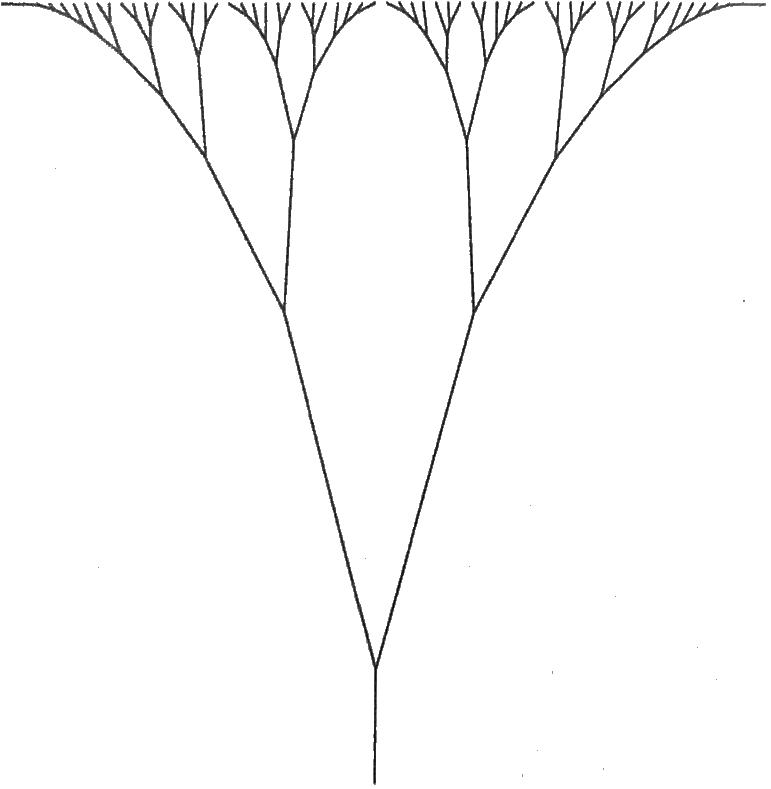
\includegraphics[scale=0.7]{graphics/johdanto_branched.png}
    \caption{Approksimaatio erään massansiirto-ongelman ratkaisulle, kun tavoitteena on siirtää massaa yhdestä pisteestä janalle. \cite[s. 166]{optimal}}
    \label{fig:branched}
\end{figure}

Energian minimoivat liikennesuunnitelmat tulevat olemaan rakenteeltaan \textit{haarautuneita} (\textit{branched}). Esimerkki haarautuneesta ratkaisusta on kuvassa \ref{fig:branched}, jossa on ollut ongelmana siirtää massa yhdestä pisteestä jollekin janalle. Haarautuneisuus tai puumaisuus on intuitiivinen lopputulos, jos oletetaan kahden pienemmän tien olevan energiatehokkaampi vaihtoehto yhden suuremman sijaan. Tätä väitettä käsittelee tarkemmin tämän tutkielman päälähdeteoksena ollut kirja \cite{optimal}.







%%%%%%%%%%%%%%%%%%%%%%%%%%%%%%%%%%%%%%%%%%%%%%%%%
%%%% Esitiedot
\chapter{Esitiedot}
Merkitään positiivisten reaalilukujen joukkoa $\Rp = [0, \infty[$. Tässä kappaleessa esitellään tarvittavat määritelmät ja tulokset, joiden pohjalle tutkielma rakennetaan. 
\section{Metriset avaruudet}

Avaruus on metrinen, jos joukon kahden alkion etäisyys toisistaan pystytään määrittämään sopivalla etäisyysfunktiolla. Etäisyysfunktiolle asetetaan seuraavat ehdot.

\begin{definition}
    Joukon $X$ funktio $d: X\times X \to \R^+$ on \textit{etäisyys} joukossa $X$, jos kaikilla $x, y, z \in X$ pätee
    \begin{enumerate}
        \item $d(x,y) = 0 \iff x = y$,
        \item $d(x,y) = d(y,x)$,
        \item $d(x,y) \le d(x,z) + d(z,y)$.
    \end{enumerate}
    Joukossa $X$ määritellystä etäisyydestä käytetään merkintää $d_X$, tai $d$ jos etäisyys on kontekstista selvä. 
\end{definition}

\begin{definition}
    Olkoon $M$ joukko ja $d$ etäisyys joukossa $M$. Tällöin pari $(M, d)$ on \textit{metrinen avaruus}, merkitään $M = (M, d)$.
\end{definition}

Joukon halkaisija määritellään joukon kahden alkion suurimman mahdollisen etäisyyden supremunina.
\begin{definition}
    Olkoon $(M, d)$ metrinen avaruus ja $A \subset M$. Joukon $A$ \textit{halkaisija} $\diam(A)$ on
    tällöin
    \begin{equation*}
        \diam(A) = \sup\{d(x, y) : x,y \in A\}.
    \end{equation*}
\end{definition}
Seuraava Cauchyn jonon määritelmä mukailee lähdettä  \cite[s. 52]{rudin}. Jonoa kutsutaan Cauchyn-jonoksi, jos jonon edetessä alkiot pääsevät mielivaltaisen lähelle toisiaan.

\begin{definition}
    Jono $(p_n)$ metrisessä avaruudessa $M$ on \textit{Cauchyn jono}, jos kaikilla $\varepsilon > 0$ on olemassa $N\in \mathbf{\N}$ siten, että $d(p_n, p_m) < \varepsilon$ jos $n, m\ge N$.
\end{definition}

Täydelliseksi metriseksi avaruudeksi kutsutaan sellaista avaruutta, johon ei jää reikiä. Esimerkiksi metrinen avaruus, joka saadaan kun reaaliluvut varustettuna tavallisella euklidisella normilla on täydellinen. Määritellään tarkasti, mitä tarkoittaa joukon täydellisyys. Motivaatio täydellisyyden määritelmään löytyy lähteestä \cite[s. 54]{rudin}.

\begin{definition}
    Metrinen avaruus on \textit{täydellinen}, jos avaruuden jokainen Cauchyn jono suppenee. 
\end{definition} 

Metrisen avaruuden peitteeksi kutsutaan kokoelmaa joukkoja, joiden yhdisteeseen avaruuden alkiot kuuluvat.

\begin{definition}
    Olkoon $I$ indeksijoukko. Metrisen avaruuden $M$ joukkojen kokoelma $C = \{C_i \subset M \colon i \in I\}$ on joukon $A \subset M$ peite, jos 
    \begin{equation*}
        A \subset \bigcup_{i\in I}C_i.
    \end{equation*}
    Peitteen $C$ osapeite on joukon $C$ osajoukko, joka edelleen peittää joukon $A$. Peite $C$ on avoin peite, jos peittämiseen käytetyt joukot $C_i$ ovat avoimia. 
\end{definition}

\begin{definition}
    Metrinen avaruus $M$ on \textit{kompakti}, jos jokaisella avaruuden $M$ avoimella peitteellä on äärellinen osapeite. 
\end{definition}

\begin{definition}
    Olkoon $(M, d)$ metrinen avaruus, $x \in M$ ja $r > 0$. Avaruuden $M$ $r$-säteinen $x$-keskinen pallo on tällöin joukko
    \begin{align*}
        B(x, r) = \{y \in M : d(x, y) < r\}.
    \end{align*}
\end{definition}

\begin{definition}
    Metrisen avaruuden $(M, d)$ joukko $A \subset M$ on \textit{tiheä} avaruudessa $M$, jos kaikille $x \in M$ ja $r > 0$ pätee $B(x, r) \cap S \ne \emptyset$, toisin sanoen kaikki avaruuden $(M, d)$ avoimet pallot sisältävät pisteen joukosta $S$.
\end{definition}

\begin{definition}
    Metrinen avaruus $M$ on \textit{täysin rajoitettu}, jos kaikilla $\varepsilon > 0$ on olemassa äärellinen kokoelma avoimia $\varepsilon$-säteisiä palloja avaruudessa $M$, joiden yhdiste sisältää avaruuden $M$.
\end{definition}

\begin{theorem}\label{thm:compactness}
    Jos metrinen avaruus $M$ on täysin rajoitettu ja täydellinen, niin se on kompakti.
\end{theorem}
\begin{proof}
Todistuksen idea on saatu verkkolähteestä \cite{gibara}.

Olkoon $(M, d)$ täysin rajoitettu ja $C$ avoin joukon $M$ peite. Osoitetaan väite käänteisellä päättelyllä. Oletetaan, että ei ole olemassa äärellistä peitteen $C$ osapeitettä.

Koska $M$ on täysin rajoitettu, se voidaan peittää 1-säteisillä palloilla. Tällöin on olemassa pallo $B(x_0,1)$, jota ei voi peittää peitteen $C$ äärellisellä osapeitteellä.

Pallo $B(x_0,1)$ voidaan peittää $1/2$-säteisillä palloilla, joiden keskipiste on korkeintaan etäisyyden $1 + 1/2$ päästä pisteestä $x_0$. Jälleen on olemassa pallo $B(x_1, 1/2)$, jota ei voi peittää peitteen $C$ äärellisellä osapeitteellä.

Vastaavasti pallo $B(x_1, 1/2)$ voidaan peittää $1/4$-säteisillä palloilla, joiden etäisyys on korkeintaan $1+1/4$ pisteestä $x_1$. Jatkamalla tähän tapaan voidaan muodostaa jono pisteitä $(x_n)$ joukossa $M$ siten, että yhtäkään palloa $B(x_n, 2^{-n})$ ei voi peittää peitteen $C$ äärellisellä osapeitteellä. Lisäksi $d(x_n, x_{n+1})  \le 2^{-n} + 2^{-n-1}$ kaikille $n$, jolloin jono $(x_n)$ suppenee. Merkitään $x = \lim_{n\to\infty} x_n$.

Olkoon joukko $A \in C$, jolle $x \in A$. Tällöin on olemassa $r > 0$ siten, että $B(x,r) \subset A$. Koska $x = \lim_{n\to\infty} x_n$, on olemassa $N$, jolle pallo $B(x_N, 2^{-N})$ sisältyy palloon $B(x, r)$. Tällöin $B(x_N, 2^{-N}) \subset B(x, r) \subset A \in C$. Siispä pallo $B(x_N, 2^{-N})$ pystytään peittämään peitteen $C$ osapeitteellä, mikä on ristiriita.
\end{proof}

Määritellään yleisesti käytetty etäisyys funktioiden avaruuteen.
\begin{definition}
Olkoon $X\subset \R^n$ ja $M$ metrinen avaruus. Funktion $f: X \to M$ \textit{sup-normi} määritellään luvuksi
\begin{equation*}
    ||f||_\infty = \sup\{|f(x)| : x \in X\}.
\end{equation*}
Joukossa $A\subset M$ äärellisiä sup-normin arvoja saavien funktioiden avaruutta merkitään
    \[L^\infty (A) = \{f:A\to M \colon  ||f||_\infty < \infty\}.\] 
Merkinnällä $||f||_{L^\infty(B)}$ rajoitetaan funktion määrittelyjoukon tarkastelu joukkoon $B$.
\end{definition}

\subsection{Jatkuvuus}
Olkoon $(X, d_x)$ ja $(Y, d_y)$ metrisiä avaruuksia. Määritellään tarvittavat jatkuvuuden käsitteet.

\begin{definition}Funktio $f: X \to Y$ on jatkuva pisteessä $x_0 \in X$, jos kaikilla $\varepsilon > 0$ on olemassa $\delta > 0$ siten, että
\begin{equation*}
    d_y(f(x), f(x_0)) < \varepsilon, \text{ kun } d_x(x, x_0) < \delta.
\end{equation*}
Merkitään jatkuvien funktioiden $f: X \to Y$ kokoelmaa $C(X, Y)$ tai $C(X)$.
\end{definition}

\begin{definition}
    Olkoon metriset avaruudet $(X, d_x)$ ja $(Y, d_y)$. Sanotaan, että funktio  ${f:X\to Y}$ on \textit{K-Lipschitz-jatkuva}, jos on olemassa $K\ge 0$ siten, että kaikille $x_1,x_2 \in X$ pätee
    $$d_y(f(x_1),f(x_2)) \le Kd_x(x_1,x_2).$$
\end{definition}

\begin{definition}
Funktioiden $f:X \to Y$ kokoelma $F$ on \textit{tasajatkuva pisteessä} $x_0 \in X$, jos kaikilla $\varepsilon > 0 $ on olemassa $\delta > 0$ siten, että $d(f(x_0), f(x)) < \varepsilon$ kaikille $f \in F$ ja kaikille $x \in X$ joille $d(x_0, x) < \delta $. Kokoelma $F$ on $tasajatkuva$, jos $F$ on tasajatkuva kaikilla $x \in X$.
\end{definition}

\begin{definition}
    Olkoon $I$ indeksijoukko. Kokoelma $F = \{f_i : X \to Y \ | \ i \in I\}$ on \textit{tasaisesti rajoitettu}, jos on olemassa $a \in Y$ ja $M \in \R$ siten, että
    \begin{equation*}
        d(f_i(x), a) \le M
    \end{equation*} 
    kaikilla $i \in I$ ja $x \in X$.
    Kokoelma reaaliarvoisia funktioita $F$ on tasaisesti rajoitettu, jos jokainen kokoelman $F$ funktio on rajoitettu samalla vakiolla $M$.
\end{definition}

\begin{theorem}\label{thm:ascoli-arzela}
    Olkoon kokoelma funktioita $F \subset C(\Rp)$, jotka on määritelty suljetulla välillä $[a, b]$. Tällöin $(F, ||\cdot||_\infty)$ on täysin rajoitettu jos ja vain jos se on tasajatkuva ja tasaisesti rajoitettu.
\end{theorem}
\begin{proof}
    Todistettu lähteessä \cite[s. 158]{rudin}. Väite tunnetaan myös Arzelan-Ascolin lauseena.
\end{proof}

\begin{definition}
    Olkoon $X\subset \R^n$. Funktio $f: X \to \R \cup\{-\infty, \infty\}$ on \textit{alhaalta puolijatkuva} pisteessä $x_0$ jos 
    $$\liminf_{x\to x_0}  f(x) \ge f(x_0).$$
\end{definition}

\begin{definition}
    Olkoon $X\subset \R^n$. Funktio $f: X \to \R \cup\{-\infty, \infty\}$ on \textit{ylhäältä puolijatkuva} pisteessä $x_0$ jos 
    $$\limsup_{x\to x_0}  f(x) \le f(x_0).$$
\end{definition}

\begin{lemma}\label{le:LSCisLimitOfC-Functions}
    Jokainen alhaalta puolijatkuva funktio $f$ kompaktissa metrisessä avaruudessa on jatkuvien funktioiden kasvavan jonon raja-arvo.
\end{lemma}
\begin{proof}
    Todistus mukailee lähteen \cite[s. 30]{optimal} todistusta. Olkoon $K$ kompakti metrinen avaruus ja $f:K \to \R$ alhaalta puolijatkuva. Asetetaan $$f_k(x) := \inf_y\{f(y) + kd(x,y)\}.$$ Tällöin $f_k$ on jatkuva kaikilla $k$ ja selvästi $f_1 \le f_2 \le ... \le f$. Osoitetaan, että kaikilla $x\in K$ pätee $f_k(x) \to f(x)$ kun $k \to \infty$. 
    Olkoon $x\in K$. Koska $K$ on kompakti, on olemassa suppeneva jono pisteitä $y_{x,i} \in K$, joille
    \begin{equation*}
        f_k(x) = \lim_{i \to \infty}(f(y_{x,i}) + k d(x, y_{x,i})).
    \end{equation*}
    Määritellään jono 
    \begin{equation*}
        x_k = \lim_{i\to \infty} y_{x,i}.
    \end{equation*}
    Osoitetaan, että $x_k \to x$, kun $k \to \infty$. Koska $f$ on alhaalta puolijatkuva, niin 
    \begin{align*}
        f(x_k) = f\left(\lim_{i\to \infty} y_{x,i}\right) \le \liminf_i (f(y_{x.i})),
    \end{align*}
    joten 
    \begin{equation*}
        f(x_k) + k d(x, x_k) \le \liminf_i (f(y_{x.i}) + k(d(x,y_{x,i})) = f(x).
    \end{equation*}
    Koska lisäksi $f_k(x) \le f(x_k) + kd(x, x_k)$ funktion $f_k$ määritelmän nojalla, niin tällöin $f_k(x) = f(x_k) + kd(x,x_k)$. Saadaan
    
    \begin{align}\label{eq:LSCIsLimit3}
        f(x) \ge f_k(x) = f(x_k) + kd(x, x_k) \ge m + k d(x, x_k),
    \end{align}
    sillä funktio $f$ on alhaalta rajoitettu jollakin vakiolla $m \in \R$. Jos näin ei olisi, löytyisi kompaktiuden nojalla jono $(z_i)$ siten, että $f(z_i) \to -\infty$, ja jonon $(z_i)$ suppenevan osajonon rajapisteessä $z$ olisi $f(z) = -\infty$ alhaalta puolijatkuvuuden nojalla. Funktio määriteltiin reaaliarvoiseksi, joten päädytään ristiriitaan. Jatkaen yhtälöstä \eqref{eq:LSCIsLimit3} saadaan 
    \begin{equation*}%\label{eq:LSCisLimit2}
        d(x, x_k) \le \frac{1}{k}(f(x) - m) \to 0
    \end{equation*}
    kun $k \to \infty$. Siispä $x_k \to x$.
    
    Lopulta funktion $f$ alhaalta puolijatkuvuudella saadaan
    \begin{align*}
        \liminf_k f_k(x) &= \liminf_k (f(x_k) + d(x,x_k)) \\
        &\ge \liminf_k f(x_k) \\
        & \ge f(x).
    \end{align*}
    Koska lisäksi $f_k \le f$, niin
    \begin{align*}
        f(x) \le \liminf_k f_k(x) \le f(x),
    \end{align*}
    joten $f_k \to f$, kun $k \to \infty$.
\end{proof}


\begin{lemma}\label{le:openPreimageImpliesUSC}
    Olkoon $f:X \to \Rp$. Jos $f^{-1}([0, r[)$ on avoin kaikilla $r > 0$, niin $f$ on ylhäältä puolijatkuva joukossa $[0, r[$.
\end{lemma}
\begin{proof}
    Olkoon $x \in X$. Kaikilla $r > 0$ joukko $f^{-1}([0, f(x) + r[)$ on avoin. Siispä kaikilla $r > 0$ on olemassa $d > 0$ s. e. $B(x, d) \subset f^{-1}([0, f(x) + r[)$, jolloin $f(B(x,d)) \subset [0, f(x) + r[$.
    
    Olkoon jono $(x_i)$ jolle $x_i \to x$. Tällöin kaikille $r > 0$ on olemassa $N_r \in \N$, jolle
    \begin{align*}
        f(x_i) \in f(B(x, d)) \subset [0, f(x) + r[,
    \end{align*}
    kaikilla $i \ge N_r$ ja jollakin $d > 0$, joten
    \begin{align*}
        0 \le f(x_i) < f(x) + r
    \end{align*}
    kaikilla $i \ge N_r$. Siispä $f(x_i) \le f(x)$ kaikilla $i \ge N_r$, joten
    \begin{align*}
        \limsup_{i\to \infty}f(x_i) \le f(x).
    \end{align*}
\end{proof}


\section{Mittateoriaa}
\subsection{Sigma-algebra}
Merkitään $2^A$ joukon $A$ osajoukkojen kokoelmaa. Seuraavat määritelmät liittyen sigma-algebraan ja Borelin joukkoihin on muotoiltu lähteeseen \cite[s. 86-87]{lehrbäck} pohjaten.

\begin{definition}
    Olkoon $X$ joukko. Tällöin $\Gamma \subset 2^X$ on \textit{sigma-algebra}, joukossa $X$, jos $\Gamma$ toteuttaa seuraavat ominaisuudet:
    \begin{enumerate}
        \item $\emptyset \in \Gamma$ 
        \item jos $A \in \Gamma$, niin $A^c \in \Gamma$
        \item jos $A_1, A_2, ... \in \Gamma$, niin $\bigcup_{j=1}^\infty A_j \in \Gamma$ 
    \end{enumerate}
    %(Lehrbäck, MII, s. 86)
\end{definition}


\begin{definition}
    Olkoon $X$ joukko ja olkoon $\Delta \subset 2^X$. Tällöin 
        $$ \Gamma_\Delta = \bigcap \{\Gamma : \Gamma \text{ on sigma-algebra joukossa } X \text{ ja }  \Delta \subset \Gamma \}$$ 
    on joukkoperheen $\Delta$ \textit{virittämä} sigma-algebra joukossa $X$.
    %(Lehrbäck, MII, s. 86)
\end{definition}

\begin{definition}
    Olkoon $X$ metrinen avaruus, ja 
    \[\Delta = \{A \subset X : A \text{ on avoin joukko}\} \subset 2^X. \]
    Tällöin $\sigma$-algebra $\mathcal B := \Gamma_\Delta$ on avaruuden $X$ \textit{Borelin sigma-algebra} ja joukkoja $A\in \mathcal B$ kutsutaan \textit{Borel-joukoiksi.} 
    %(Lehrbäck, MII, s.87, muokattu)
\end{definition}

Sigma-algebran $\Gamma_\Delta$ määritelmän nojalla Borelin sigma-algebra on \textit{suppein} avoimista joukoista koostuva joukon $X$ sigma-algebra, joka sisältää joukkoperheen $\Delta$. 

\begin{definition}
    Olkoon $X\subset \R^n$ joukko ja $\mathcal{B}$ Borelin sigma-algebra joukossa $X$. Tällöin pari $(X, \mathcal{B})$ on \textit{Borelin avaruus}.
\end{definition}

\subsection{Ulkomitta ja mitta}
Mittaan ja funktion mitallisuuteen liittyvät määritelmät on mukailtu lähteen \cite[s. 88-110]{lehrbäck} avulla. Aloitetaan ulkomitan ja mitallisten joukkojen määritelmästä.
\begin{definition}
    Olkoon $X$ joukko. Funktio $\mu^*: 2^X \to \Rp$ on \textit{ulkomitta} joukossa $X$, jos pätee
    \begin{enumerate}
        \item $\mu^*(\emptyset) = 0.$
        \item Jos $A \subset B \subset X$, niin $\mu^*(A) \le \mu^*(B)$.
        \item Jos $A_1, A_2, ... \subset X$, niin 
        \begin{align*}
            \mu^*\left(\bigcup_{j=1}^\infty A_j \right) \le \sum_{j = 1}^\infty\mu^*(A_j).
        \end{align*}
    \end{enumerate}
\end{definition}

\begin{definition}
    Joukko $A\subset \R^n$ on $\mu^*$-\textit{mitallinen}, jos kaikille $E\subset \R^n$ pätee
    \begin{equation}\label{eq:measurable}
        \mu^*(E) = \mu^*(E \cap A^c) + \mu^*(E\cap A).
    \end{equation}
    %(Lehrbäck, MII, s. 27)
\end{definition}

\begin{lemma}\label{le:countableUnionAndIntersectionIsMeas}
    Mitallisten joukkojen $A_1, A_2, ...$ numeroituva yhdiste $\bigcup_{j=1}^\infty A_j$ ja numeroituva leikkaus $\bigcup_{j=1}^\infty A_j$ ovat mitallisia.
\end{lemma}
\begin{proof}
    Numeroituvan yhdisteen tapaus sivuutetaan; tämä on todistettu lähteessä \cite[s. 94]{lehrbäck}.
    De Morganin sääntöjen nojalla
    \begin{align*}
        \bigcap_{j=1}^\infty A_j = \left(\bigcup_{j=1}^\infty A_j^c\right)^c.
    \end{align*}
    Siispä numeroituva leikkaus on mitallinen, jos mitallisen joukon komplementti on mitallinen. Tämä seuraa suoraan mitallisuusehdosta \eqref{eq:measurable}.
\end{proof}

Osoittautuu, että riittävä ehto joukkojen mitallisuuden takaamiseksi on se, että joukot muodostavat sigma-algebran. Perustelu tälle on esitelty lähteessä \cite[s. 79]{tao}. Määritellään seuraavaksi mitta ja mitta-avaruus.

\begin{definition}
    Oletetaan, että $X$ on joukko ja $\Gamma$ on $\sigma$-algebra joukossa $X$. Funktio $\mu : \Gamma \to [0, \infty]$ on \textit{mitta} (joukossa X tai $\sigma$-algebrassa $\Gamma$), jos 
    \begin{enumerate}
        \item $\mu(\emptyset) = 0$, \\
        ja
        \item Jos $A_1, A_2, ... \in \Gamma$ ovat erillisiä eli $A_i \cap A_j = \emptyset$ aina, kun $i \ne i$, niin
        $$\mu\left(\bigcup_{j=1}^\infty A_j \right) = \sum_{j=1}^\infty \mu(A_j).$$
    \end{enumerate}
    
    Kolmikkoa $(X,\Gamma, \mu)$ sanotaan \textit{mitta-avaruudeksi} ja joukkoja $A\in \Gamma$ sanotaan $\Gamma$-mitallisiksi.
    
    %(Lehrbäck, MII, s. 88)
\end{definition}

Määritellään Lebesguen ulkomitta ja mitta, jonka jälkeen todistetaan tarvittava tulos sisäkkäisten joukkojen Lebesguen mitan raja-arvosta. Lebesguen mitan määritelmä on mukailtu lähteestä \cite[s. 40]{lehrbäck}.

\begin{definition}
    Avaruuden $\R^n$ \textit{avoimia välejä} ovat joukot
    \begin{align*}
        I = I^{(1)} \times I^{(2)} \times ... \times I^{(n)},
    \end{align*}
    jossa $I^{(k)} = ]a_k, b_k[ \subset \R$ joillain $a_k, b_k \in \R$.
    Välin $I$ \textit{geometrinen mitta} on
    \begin{align*}
        v(I) = \prod_{k=1}^n(b_k-a_k).
    \end{align*}
\end{definition}

\begin{definition}
    Funktio $\lambda^* : \R^n \to \R^+$ on \textit{Lebesguen ulkomitta} kun määritellään
    $$\lambda^*(A) = \inf\left\{\sum_{i=1}^\infty v(I_i) : I_i \subset \R^n \text{ on avoin väli tai tyhjä joukko, ja } A \subset \bigcup_{i=1}^{\infty}I_i\right\}$$
    kaikille $A \subset \R^n$.
\end{definition}

\begin{definition}
    Olkoon $\mathcal M$ joukon $\R^n$ mitallisten joukkojen kokoelma. Funktio $\lambda : \mathcal M \to \R^+$ on \textit{Lebesguen mitta} kun määritellään
    $$\lambda(A) = \lambda^*(A) \text{ kaikille } A \in \mathcal M.$$
\end{definition}

\begin{lemma}\label{le:nestedIntersection}
    Olkoon $A_1 \supset A_2 \supset A_3 \supset ...$ ja $A = \cap_{k=1}^\infty A_k$. Jos $\lambda(A_1) < \infty$, niin 
    \begin{equation*}
        \lambda(A) = \lim_{k\to \infty}\lambda(A_k).
    \end{equation*}
\end{lemma}
\begin{proof} Todistuksen idea on saatu verkkolähteestä \cite{brozius}.
    Määritellään apujoukko $B_n$ siten, että $B_n = A_n \setminus A_{n+1}$ kaikille $n \in \N$. Tällöin
    \begin{align*}
        A_k = A \cup \bigcup_{n = k}^\infty B_n,
    \end{align*}
    joten $A_k$ voidaan esittää kahden erillisen joukon yhdisteenä. Siispä
    \begin{align*}
        \lambda(A_k) &= \lambda(A) + \lambda\left(\bigcup_{n = k}^\infty B_n\right) \\
        &= \lambda(A) + \sum_{n = k}^\infty\lambda(B_n).
    \end{align*}
    Jos $m(A_{k_0}) < \infty$ jollekin $k_0$, niin $m(E) < \infty$ ja $\sum_{n = k}^\infty\lambda(B_n) < \infty$, joten 
    \begin{align*}
        \lim_{k\to\infty}\lambda(A_k) = \lim_{k\to\infty}\left(\lambda(A) + \sum_{n = k}^\infty\lambda(B_n)\right) = \lambda(A) + \lim_{k\to\infty}\sum_{n=k}^\infty \lambda(B_n) = \lambda(A).
    \end{align*}
\end{proof}

\begin{lemma}\label{le:lebesgueIsBorelAndNull}
    Olkoon Lebesgue-mitallinen joukko $A \subset \R^n$. Tällöin on olemassa Borelin joukko $B \subset X$ ja nollamittainen joukko $N$ siten, että $A = B \cup N$.
\end{lemma}
\begin{proof}
    Koska $A$ on Lebesgue-mitallinen, niin kaikille $\varepsilon > 0$ on olemassa suljettu joukko $B_\varepsilon \subset A$ siten, että $\lambda(A\setminus B_\varepsilon) \le \varepsilon$. Tämä väite on osoitettu lähteessä \cite[s. 43]{lehrbäck}. 
    Tällöin
    \begin{align*}
        \lambda\left(A \setminus \bigcup_{n \in \N} B_{1/n}\right) \to 0,
    \end{align*}
    kun $n \to \infty$.
    Siispä $N := A \setminus \bigcup_n B_{1/n}$ on nollamittainen. Lisäksi yhdiste $B:= \bigcup_{n}B_{1/n}$ on numeroituvana suljettujen joukkojen yhdisteenä Borel-joukko, ja $A = B \cup N$.
\end{proof}

\subsection{Funktion mitallisuus}
Määritellään funktion mitallisuus. Mitallisuuden lisäksi tarvitaan aputuloksina mitallisuusehtoja, joista tärkeimpänä on mitallisuuden seuraaminen puolijatkuvuudesta. Funktion mitallisuus metrisessä avaruudessa riippuu funktion lisäksi määrittely- ja maalijoukon avaruuksien sigma-algebroista.

\begin{definition}\label{def:measurable}
    Olkoon $(X, \Sigma)$ ja $(Y, \Gamma)$ metrisiä avaruuksia, missä $X$ ja $Y$ ovat joukkoja varustettuna sigma-algebroilla $\Sigma$ ja $\Gamma$. Funktio $f: X \to Y$ on mitallinen, jos kaikkien $E\in \Gamma$ alkukuva funktiolle $f$ sisältyy kokoelmaan $\Sigma$, toisin sanoen kaikille $E \in \Gamma$
    \begin{equation*}
        f^{-1}(E) = \{x \in X : f(x) \in E\} \in \Sigma.  
    \end{equation*}
\end{definition}
Merkinnällä $f: (X, \Sigma) \to (Y, \Gamma)$ tarkoitetaan funktiota $f:X \to Y$, jonka määrittelyjoukko on varustettu sigma-algebralla $\Sigma$ ja maalijoukko sigma-algebralla $\Gamma$.
\begin{definition}
Funktio $f:(X, \Borel_X) \to (Y, \Borel_Y)$ on Borel-mitallinen, jos funktio on mitallinen, ja $(X, \Borel_X)$ sekä $(Y, \Borel_Y)$ ovat Borelin avaruuksia.
\end{definition}
\begin{corollary}\label{co:LSCimpliesMeasurable}
    Alhaalta ja ylhäältä puolijatkuvat kuvaukset ovat Borel-mitallisia.
\end{corollary}
\begin{proof}
    Lemman \ref{le:LSCisLimitOfC-Functions} nojalla alhaalta puolijatkuva funktio voidaan esittää jatkuvien kuvausten raja-arvona. Jatkuvat kuvaukset ovat mitallisia, joten niiden raja-arvo on mitallinen. Siispä alhaalta puolijatkuva kuvaus on mitallinen. 
    
    Jos kuvaus $f$ on ylhäältä puolijatkuva, niin $-f$ on alhaalta puolijatkuva. Siispä ylhäältä puolijatkuva $f$ on myös mitallinen.
\end{proof}

\begin{lemma}
    Olkoon mitta-avaruudet $(X_1, \Gamma_1), (X_2, \Gamma_2)$ ja $(X_3, \Gamma_3)$. Olkoon funktiot $f:X_1 \to X_2$ ja $g:X_2 \to X_3$ mitallisia. Tällöin funktioiden $f$ ja $g$ yhdistetty funktio $g \circ f:(X_1, \Gamma_1) \to (X_3, \Gamma_3)$ on mitallinen.
\end{lemma}
\begin{proof}
    Olkoon $E \in \Gamma_3$. Tällöin funktion $g$ mitallisuuden nojalla $g^{-1}(E) \in \Gamma_2$, ja funktion $f$ mitallisuuden nojalla $f^{-1}(g^{-1}(E)) \in \Gamma_1$. Siispä kaikilla $E \in \Gamma_3$ pätee $(g\circ f)^{-1}(E) \in \Gamma_1$, joten $g\circ f$ on mitallinen.
\end{proof}

\begin{lemma}\label{le:measurableIfBallMeasurable}
    Olkoon $X, Y \subset \R^n$ varustettuina Borelin sigma-algebroilla $\mathcal B_X$, $\mathcal B_Y$. Kuvaus $f: (X, \mathcal B_X) \to (Y, \mathcal B_Y)$ on mitallinen, jos jokaisen avoimen pallon alkukuva funktiolle $f$ on mitallinen.
\end{lemma}
\begin{proof}
    Olkoon $E\in\mathcal B_X$ avoin. Osoitetaan, että on olemassa numeroituva avoimien pallojen yhdiste, joille
    \begin{equation*}
        E = \bigcup_i B(x_i, r_i).
    \end{equation*}
    Koska $E$ on avoin, niin kaikille $x \in E$ on olemassa $r > 0$ siten, että $B(x, r) \subset E$. Koska $X$ on tiheä avaruuden $\R^n$ osajoukkona, on olemassa $x_p \in \Q^n$ ja $x_q \in \Q$, joille $B(x_p, x_q) \subset B(x, r)$ ja lisäksi $x \in B(x_p, x_q)$. Lisäksi, koska $B(x_p, x_q) \subset E$, niin pallojen numeroituva yhdiste sisältyy joukkoon $E$.
    
    Koska oletuksen nojalla avoimen pallon alkukuva on mitallinen, pätee funktion alkukuvalle
    \begin{align*}
        f^{-1}(E) &= f^{-1}\left(\bigcup_i B(x_i, r_i)\right) \\
        &= \bigcup_i f^{-1}(B(x_i, r_i)) \in \mathcal B_X
    \end{align*}
    numeroituvana mitallisten joukkojen yhdisteenä. 
    
    Olkoon 
    \begin{align*}
        \Sigma =\{A \subset Y : f^{-1}(A) \in \mathcal B_x\},
    \end{align*}
    jolloin $\Sigma$ sisältää kaikki avaruuden $Y$ joukot, joiden alkukuva on Borel-joukko. Osoitetaan, että $\Sigma$ on sigma-algebra. 
    
    Kokoelma $\Sigma$ sisältää Borelin sigma-algebran määritelmän nojalla kaikki Borel-joukot. Tällöin $\emptyset \in \Sigma$. 
    
    Olkoon $A \in \Sigma$, jolloin $f^{-1}(A) \in \mathcal B_x$. Koska $\mathcal B_x$ on sigma-algebra, niin joukon $A$ komplementille $f^{-1}(A^c) \in \mathcal B_x$. Funktion alkukuvan komplementti on komplementin alkukuva, joten $f^{-1}(A)^c = f^{-1}(A^c) \in \mathcal{B}_x$.
    
    Olkoon $A_1, A_2, ... \in \Sigma$. Tällöin $f^{-1}(A_i) \in B_x$ kaikilla $i \ge 1$. Koska yhdisteen alkukuva on alkukuvien yhdiste, niin
    \begin{equation*}
        f^{-1}\left(\bigcup_{j=1}^\infty A_j\right) = \bigcup_{j=1}^\infty f^{-1}(A_j) \in \mathcal{B}_x.
    \end{equation*}
    Siispä $\Sigma$ on sigma-algebra, ja siten $f$ on mitallinen.
\end{proof}

\begin{definition}
Olkoon $\Sigma$ sigma-algebra joukossa $X$ ja $\mu:\Sigma \to [0,1]$ mitta joukossa $X$. Jos $\mu(X) = 1$, niin tällöin $\mu$ on \textit{todennäköisyysmitta} joukossa $X$, merkitään $\mu \in \mathcal{P}(X)$. 
    Jos mitta on todennäköisyysmitta, käytetään mitasta myös nimitystä \textit{yksi-massainen.}
\end{definition}

Määritellään reaaliarvoiselle funktiolle mitallisuus. Määritelmä on reaaliarvoiselle funktiolle ekvivalentti Määritelmän \ref{def:measurable} kanssa, mutta tämän väitteen osoittaminen sivuutetaan. Yhtäpitävyys seuraa siitä, että mikä tahansa avoin väli pystytään muodostamaan numeroituvalla määrällä operaatioita väleille $]a, \infty]$, kun $a \in \R$.

\begin{definition}
     Olkoon $X$ joukko ja $\Gamma \subset 2^X$ sigma-algebra. Olkoon $A\in \Gamma$. Funktio $f: A \to \R \bigcup\{-\infty, \infty\}$ on ($\Gamma$)-mitallinen, jos kaikille $a \in \R$ pätee, että
    \begin{equation*}
        \{x \in A : f(x) > a\} = f^{-1}(]a, \infty]) \in \Gamma.
    \end{equation*} 
    Jos $\mu:\Gamma \to \Rp$ on mitta ja $f$ on $\Gamma$-mitallinen, sanotaan, että $f$ on $\mu$-mitallinen.
    %(Lehrbäck MII, s. 110)
\end{definition}

Reaaliarvoisen funktion mitallisuus on yhtäpitävää myös seuraavien ehtojen kanssa.
\begin{lemma}
    Olkoon $X$ joukko, $\Gamma$ sigma-algebra joukossa $X$ ja reaaliarvoinen funktio $f : X \to \R \cup \{-\infty, \infty\}$. Tällöin seuraavat ehdot ovat yhtäpitäviä:
    \begin{enumerate}
        \item $f$ on mitallinen
        \item $f^{-1}([a, \infty[) \in \Gamma $ kaikilla $a \in \R$
        \item $f^{-1}(]-\infty, a])\in \Gamma $ kaikilla $a \in \R$
        \item $f^{-1}(]-\infty, a[)\in \Gamma $ kaikilla $a \in \R$.
    \end{enumerate}
\end{lemma}
\begin{proof}
    Todistus sivuutetaan. Todistettu Lebesgue-mitalle ja -mitallisille joukoille lähteessä \cite[s. 52]{lehrbäck}. Esiteltyjen ehtojen yhtäpitävyys todistetaan vastaavasti.
\end{proof}
\subsection{Integraali ja integroituvuus}
Seuraavat määritelmät liittyen yleiseen mitta-avaruuden integraaliin ja integroituvuuden on mukailtu lähteestä \cite[s. 110-111]{lehrbäck}. 
\begin{definition}
    Olkoon $\Gamma \subset 2^X$ sigma-algebra. Funktio $u: X \to \R$ on $\Gamma$-\textit{yksinkertainen}, merkitään $u \in Y_\Gamma$, jos
    \begin{align*}
        u(x) = \sum_{i=1}^M a_i \indfct{A_i}(x) \quad \text{kaikille } x \in X,
    \end{align*}
    missä $a_i \in \R$ ja $A_i \in \Gamma$ kaikille $i = 1, ..., M.$ Jos $u \in Y_\Gamma$ ja $u(x) \ge 0$ kaikille $x \in X$, niin merkitään, että $u \in Y_\Gamma^+$.
\end{definition}

\begin{lemma}
    Jokaisella $u \in Y_\Gamma$ on normaaliesitys, jolloin $a_i \ne a_j$ ja $A_i \cap A_j = \emptyset$ aina, kun $i \ne j$.
\end{lemma}
\begin{proof}
    Todistettu lähteessä \cite[s. 110]{lehrbäck}.
\end{proof}

\begin{lemma}
    Funktio $f: A \to [0, \infty]$ on $\Gamma$-mitallinen jos ja vain jos on olemassa yksinkertaiset funktiot $u_k \in Y_\Gamma^+$ siten, että $u_k \le u_{k+1}$ kaikille $k \in \N$ ja $\lim_{k\to\infty}u_k(x) = f(x)$ kaikille $x \in A$.
\end{lemma}
\begin{proof}
    Todistettu lähteessä \cite[s. 110]{lehrbäck}.
\end{proof}

\begin{definition}
    Olkoon funktion $u \in Y_\Gamma^+$ normaaliesitys $u(x) = \sum_{i=1}^M a_i\indfct{A_i}(x)$ ja olkoon $E \in \Gamma$. Tällöin funktion $u$ yksinkertainen $\mu$-integraali yli joukon $E$ on
    \begin{equation*}
        I(u, E; \mu) = \sum_{i=1}^M a_i \mu(A_i \cap E).
    \end{equation*}
\end{definition}

\begin{definition}
    Olkoon $(X, \Gamma, \mu)$ mitta-avaruus. Jos $f: A \to [0, \infty]$ on $\Gamma$-mitallinen, niin funktion $f$ $\mu$-integraali yli joukon $A$ on
    \begin{align*}
        \int_A f \, d\mu = \sup\{I(u, A; \mu) : u \in Y_\Gamma^+, u(x) \le f(x) \text{ kaikille } x \in A\}.
    \end{align*}
\end{definition}

\begin{definition}
    $\Gamma$-mitallinen funktio $f$ on $\mu$-integroituva yli joukon $A$, mikäli $\int_A f^+ \, d\mu < \infty$ ja $\int_A f^-\, d\mu < \infty$, kun $f^+$ ja $f^-$ ovat funktion $f$ positiivi- ja negatiiviosat.
\end{definition}
Mikäli mitta $\mu$ ja joukko $A$ ovat kontekstista selvät, sanotaan pelkästään, että $f$ on integroituva.

Yleisen mitta-avaruuden integraalille pätevät samat perusominaisuudet, kuten Lebesgue-integraalille. Näiden ominaisuuksien todistus sivuutetaan.
\begin{lemma}\label{le:integralProperties}
    Olkoon $(X, \Gamma, \mu)$ mitta-avaruus ja olkoon $A\in \Gamma$. Oletetaan, että funktiot $f, g$ ovat $\mu$-integroituvia yli joukon $A$ ja $\lambda \in \R$. Tällöin
    \begin{enumerate}
        \item $\lambda f$ on $\mu$-integroituva yli joukon $A$, ja 
        \begin{equation*}
            \int_A \lambda f \, d\mu = \lambda \int_A f \, d\mu.
        \end{equation*}
        \item $f + g$ on $\mu$-integroituva yli joukon $A$, ja
        \begin{equation*}
            \int_A  (f+g) \, d\mu = \int_A  f \, d\mu + \int_A  g \, d\mu.
        \end{equation*}
        \item jos $\gamma$-mitalliset joukot $A_j \subset A, j = 1, 2, ...$ ovat erillisiä, niin
        \begin{equation*}
            \int_{\cup_{j=1}^\infty A_j}f \, d\mu = \sum_{j=1}^\infty \int_{A_j} f\, d\mu.
        \end{equation*}
        \item jos $f(x) \le g(x)$ $\mu$-melkein kaikille $x \in A$, niin 
        \begin{equation*}
            \int_A f \, d\mu \le \int_A g \, d\mu.
        \end{equation*}
    \end{enumerate}
\end{lemma}
\begin{proof}
    Todistetaan, kuten Lebesgue-integraalille, ks. \cite[s. 113]{lehrbäck}.
\end{proof}

Tärkeässä osassa tulee esiintymään monotonisen konvergenssin lause, joka antaa ehdot sille, milloin funktiojonon alkioiden integraalien raja-arvo on raja-arvon integraali.
\begin{theorem} \label{thm:monoConvThm}
    Olkoon $(X, \mathcal{B}, \mu)$ mitta-avaruus ja olkoot $f_n:X\to [0, \infty]$ mitallisia funktioita siten, että funktiojono $(f_k)$ on kasvava. Tällöin
    \begin{equation*}
        \lim_{n\to\infty} \int_X f_n \, d\mu = \int_X \lim_{n\to \infty} f_n \, d\mu.
    \end{equation*}
\end{theorem}
\begin{proof}
    Todistettu lähteessä \cite[s. 107]{tao}.
\end{proof}

\begin{theorem}\label{thm:markov}
    Olkoon $(X, \Gamma, \mu)$ mitta-avaruus ja $f$ $\Gamma$-mitallinen funktio, kun $A \in \Gamma$. Tällöin
    \begin{equation*}
        \mu(\left\{x \in A : |f(x)| \ge t\right\}) \le \frac{1}{t}\int_A |f| \, d\mu
    \end{equation*}
    kaikilla $t\in \Rp$.
\end{theorem}
\begin{proof}
    Todistuksen idea on saatu verkkolähteestä \cite{markov}. Tulos tunnetaan myös nimellä Markovin epäyhtälö.
    
    Olkoon $t \in \Rp$ ja merkitään
    \begin{equation*}
        B = \{x \in A : |f(x)| \ge t\}.
    \end{equation*}
    Olkoon $\indfct{B}: B \to A$ indikaattorifunktio. Osoitetaan, että kaikilla $x\in A$ pätee $t\indfct{B}(x) \le |f(x)|$. Olkoon $x \in A$. Jos $x \in B$, niin 
    \begin{equation*}
        t\indfct B (x) = t \le |f(x)|,
    \end{equation*}
    ja jos $x \notin B$, niin
    \begin{equation*}
        t\indfct B (x) = 0 \le |f(x)|.
    \end{equation*}
    Siispä kaikilla $x\in A$ on $t\indfct{B}(x) \le |f(x)|$.
    
    Integroitavan funktion integraalin monotonisuuden, eli Lemman $\ref{le:integralProperties}$ nojalla
    \begin{equation}\label{eq:markov1}
        \int_A t\indfct{B} \, d\mu \le \int_A |f| \, d\mu,
    \end{equation}
    ja toisaalta
    \begin{equation}\label{eq:markov2}
        \int_A t\indfct{B} \, d\mu = t\int_A \indfct{B} \, d\mu, = t\mu(B).
    \end{equation}
    Yhdistämällä tulokset \eqref{eq:markov1} ja \eqref{eq:markov2}, saadaan
    %\begin{align*}
        $\mu(B) \le \frac{1}{t}\int_A |f| \, d\mu.$
    %\end{align*}
\end{proof}

\begin{definition}
    Olkoon Borelin avaruudet $(X_1, \Borel_1)$ ja $(X_2, \Borel_2)$, mitallinen funktio $f:X_1 \to X_2$ ja mitta $\mu: \Borel_1 \to \R^+$. Mitan $\mu$ \textit{pusku} on mitta $f_\#\mu: \Borel_2 \to \R^+$, kun määritellään
    $$f_\# \mu (B) = \mu(f^{-1}(B)) \text{ kaikilla } B\in \Borel_2.$$
\end{definition}
Mitan $\mu$ puskun määritelmää on havainnollistettu kuvassa \ref{fig:push-forward}. Puskun määritelmää tarvitaan reaalifunktioista tutun muuttujanvaihtolauseen vastineeseen mitta-avaruuksissa.

\begin{figure}
    \centering
    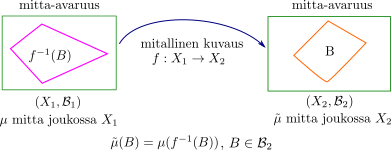
\includegraphics{graphics/push-forward.png}
    \caption{Puskun määritelmän havainnollistus. Mitallisen funktion $f: (X_1, \Borel_1) \to (X_2, \Borel_2)$ puskeminen joukon $X_1$ määritellään joukon $X_2$ mittana $\tilde \mu$.}
    \label{fig:push-forward}
\end{figure}

\begin{theorem}\label{thm:push-cov}
    Olkoon Borelin avaruudet $(X_1, \Borel_1)$ ja $(X_2, \Borel_2)$, mitalliset kuvaukset $f: X_1 \to X_2$ ja $g: X_2 \to \R^+$, sekä mitta $\mu:\Borel_1 \to [0, \infty]$. Mikäli $g$ on $f_\#\mu$-integroituva, niin  $g \circ f$ on $\mu$-integroituva. Lisäksi
    \begin{equation*}
        \int_{X_2} g \, d(f_{\#} \mu) = \int_{X_1} g \circ f \, d\mu.
    \end{equation*}
\end{theorem}
\begin{proof}
Todistettu lähteessä \cite[s. 190]{bogachev}.
\end{proof}



\subsection{Heikko suppeneminen} 

\begin{definition}
    Olkoon funktio $f:X \to \R$, missä $X$ on metrinen avaruus. Funktion $f$ kantaja $\supp(f)$ on sulkeuma funktion $f$ määrittelyjoukon osajoukosta, jossa funktio $f$ saa nollasta poikkeavia arvoja, eli
    \begin{equation*}
        \supp(f) = \overline{\{x \in X : f(x) \ne 0\}}.
    \end{equation*}
     Jos funktion $f$ kantaja on kompakti, merkitään $f \in C_c(X)$.
\end{definition}

\begin{definition} \label{def:weakConv}
    Olkoon $\P \in \mathcal{P}(K)$ mitta metrisessä avaruudessa $(X, d)$. Mittojen $\P_n \in \mathcal{P}(K)$ jono $(\P_n)$ suppenee heikosti, merkitään $\P_n \rightharpoonup \P$, jos pätee 
    \begin{equation*}
        \lim_{n\to\infty} \int_X f(x) \, d\P_n (x) = \int_X f(x) \, d\P(x)
    \end{equation*}
    kaikilla $f \in C_c(X)$.
\end{definition}

Seuraava tulos tunnetaan myös nimellä Rieszin esityslause.

\begin{theorem}\label{thm:Riesz}
    Olkoon $X$ kompakti metrinen avaruus. Olkoon $\kappa:C_c(X) \to \R$ positiivinen ja lineaarinen funktionaali. Tällöin on olemassa sigma-algebra $\Sigma$, joka sisältää kaikki Borelin joukot joukossa $X$ ja on olemassa yksikäsitteinen positiivinen mitta $\mu:\Sigma \to \Rp$, jolle
    \begin{align*}
        \kappa (f) = \int_X f \, d\mu \text{ kaikille } f \in C_c(X).
    \end{align*}
\end{theorem}
\begin{proof}
    Todistus sivuutetaan, todistettu lähteessä \cite[s. 40]{rudin}.
\end{proof}

\begin{theorem}\label{thm:probmeasureconvergence}
    Olkoon $K$ kompakti metrinen avaruus ja $(\mu_n)$ jono todennäköisyysmittoja joukossa $K$. Tällöin jonolla $(\mu_n)$ on heikosti suppeneva osajono.
\end{theorem}
\begin{proof}
    Olkoon $f \in C_c(X, \R)$. Merkintöjen helpottamiseksi merkitään $\mu(f) = \int f \, d\mu$. Koska $X$ on kompakti, on $C_c(X, \R)$ \textit{separoituva}, eli on olemassa numeroituva tiheä osajoukko funktioita $\{f_i\}_{i = 1}^\infty \subset C_c(X)$ \cite[s. 140]{conway}. Tällöin reaalilukujen jonolle $(\mu_n(f_1))$ pätee
    \begin{equation}
        |\mu_n(f_1)| \le ||f_1||_\infty,
    \end{equation}
    kaikille $n$, joten $(\mu_n(f_1))$ on rajoitettu reaalilukujono. Tällöin sille on olemassa suppeneva osajono, merkitään $(\mu_n^{(1)}(f_1))$.
    
    Tutkitaan seuraavaksi jonoa $(\mu_n^{(1)}(f_2))$, joka on jälleen rajoitettu reaalilukujono, jolla on suppeneva osajono $(\mu_n^{(2)}(f_2))$.
    
    Tähän tapaan saadaan kaikille $i \ge 1$ sisäkkäiset jonot $\{\mu_n^{(i)}\} \subset \{\mu_n^{(i-1)}\}$ joille $(\mu_n^{(i)}(f_j))$ suppenee kaikilla $1 \le j \le i$. Tarkastellaan diagonaalista jonoa $(\mu_n^{(n)})$. Koska kaikille $n \ge i$ jono $(\mu_n^{(n)})$ on jonon $(\mu_n^{(i)})$ osajono, niin $(\mu_n^{(n)}(f_i))$ suppenee kaikilla $i \ge 1$.
    
    Käytetään kokoelman $\{f_i\}$ tiheyttä osoittamaan, että $\mu_n^{(n)}(f)$ suppenee kaikilla $f \in C(X, \R)$. Olkoon $\varepsilon > 0$, jolloin voidaan valita $f_i$ siten, että $||f-f_i||_\infty \le \varepsilon.$ Koska $\mu_n^{(n)}(f_i)$ suppenee, on olemassa $N$ siten, että 
    \begin{equation*}
        |\mu_n^{(n)}(f_i) - \mu_m^{(m)}(f_i)|\le \varepsilon
    \end{equation*}
    kaikilla $n, m \ge N$. Siispä
    \begin{align*}
        |\mu_n^{(n)}(f) - \mu_m^{(m)}(f_i)| &=  |\mu_n^{(n)}(f) - \mu_n^{(n)}(f_i) + \mu_m^{(m)}(f_i) - \mu_m^{(m)}(f_i) \\ &\quad  + u_n^{(n)}(f_i) - u_m^{(m)}(f_i) | \\
        &\le |\mu_n^{(n)}(f) - \mu_n^{(n)}(f_i)| + |\mu_m^{(m)}(f_i) - \mu_m^{(m)}(f_i)| \\ &\quad  + |u_n^{(n)}(f_i) - u_m^{(m)}(f_i) | \\
        &\le 3\varepsilon
    \end{align*}
    kun $n, m \ge N$, joten $\mu_n^{(n)}(f)$ suppenee. Määritellään $w(f) = \lim_{n \to \infty} \mu_n^{(n)}(f)$. Osoitetaan, että $w$, on lineaarinen ja positiivinen, jolloin Rieszin esityslauseen $\ref{thm:Riesz}$ oletukset täyttyvät. 
    
    Kuvaus $w$ on lineaarinen, sillä kun $A, B \in \R$, niin
    \begin{align*}
        w(A f + B g) &= \lim_{n \to \infty} \mu_n^{(n)}(A f + B g) \\
        &=\lim_{n \to \infty} \int (A f + B g) \, d\mu_n^{(n)} \\
        &=\lim_{n \to \infty}  \left(A \int f \, d\mu_n^{(n)} + B \int g \, d\mu_n^{(n)}\right)  \\
        &= A w(f) + B w(g).
    \end{align*}
    Koska $|w(f)| \le ||f||_\infty$ ja $f \in C_c(X, \R)$ niin $w$ on rajoitettu. Lisäksi, jos $f \ge 0$, niin tällöin selvästi $w(f) \ge 0$, joten $w$ on positiivinen.

%Lopulta kaikille $n, m$ pätee $\mu_n^{(m)} \in \mathcal P(K)$, niin $w(1) = \lim_{n\to\infty} \mu_n^{(n)}(1) = 1$, joten $w \in \mathcal P(K)$

    Siispä Lauseen \ref{thm:Riesz} nojalla on olemassa $\mu \in \mathcal P(K)$, jolle $w(f) = \int f \, d\mu$. Tällöin kaikille $f \in C(X, \R)$ on
    \begin{equation*}
        \int f \, d\mu_n^{(n)} \to \int f \, d\mu
    \end{equation*}
    kun $n \to \infty$, toisin sanoen $\mu_n^{(n)} \to \mu$ kun $n \to \infty$.
\end{proof}

%%%% Liikennesuunnitelmat
\chapter{Liikennesuunnitelmat}

Tämän tutkielman tavoitteena on rakentaa massansiirtämiseen liittyvää teoriakehystä, pääosin niin kutsuttujen \textit{liikennesuunnitelmien} avulla. Liikennesuunnitelma tullaan määrittelemään mittana Lipschitz-polkujen joukolle muutamin lisäehdoin. Lopulta osoitetaan, että on olemassa liikennesuunnitelma, joka minimoi kuljetusongelman energian, joka määritellään myöhemmin. 

\section{Poluista}
Ennen perehtymistä liikennesuunnitelmaan, määritellään massan siirtämiseen käytettävien reittien rakenne. Kuvitellaan tilanne, että halutaan siirtää tason $\R^2$ pisteestä $A$ pisteeseen $B$ paketti. Mahdollisia paketin reittejä on äärettömän monta, mutta on syytä olettaa kaikki reitit jatkuviksi. Jatkuvia kuvauksia reaaliakselilta johonkin joukon $\R^n$ osajoukkoon kutsutaan poluiksi. 

Merkitään $X \subset \R^n$. Jatkuvuutta varten määritellään joukon $X$ alkioille normi ja etäisyys Euklidisena normina.
\begin{definition}
    Alkion $x \in X$ \textit{normi} $|\cdot|$ määritellään
    \begin{equation*}
        |x| = \sqrt{x_1^2 + x_2^2 + ... + x_n^2},
    \end{equation*}
    kun $x = (x_1, x_2, ... , x_n)$. Kahden alkion $x, y \in X$ etäisyys on tällöin
    \begin{equation*}
        d(x, y) = |x - y|.
    \end{equation*}
\end{definition}

\begin{definition}
    Jatkuvaa kuvausta $\gamma:\Rp \to X$ sanotaan \textit{poluksi.}
\end{definition}

Koska polku määritellään saamaan arvoja jokaisella positiivisella $t \in \Rp$, on syytä määritellä, milloin polku pysähtyy.

\begin{definition}
    Määritellään polun $\gamma$ \textit{pysähtymisajaksi} 
    \begin{equation*}
        T(\gamma) = \inf\{t\ge0:\gamma(t) \text{ vakio välillä } [t,\infty[ \}.
    \end{equation*}
\end{definition}

\begin{definition}
    Olkoon $\gamma$ polku. Polun $\gamma$ pituus $L(\gamma)$ määritellään osapituuksien summan supremunina
    \begin{equation*}
        L(\gamma) = \sup\left\{\sum_{i=1}^N|\gamma(t_i) - \gamma(t_{i-1})| : t_1 \le t_2 \le ... \le t_N \le T(\gamma)\right\}.
    \end{equation*}
\end{definition}

\begin{definition}
    Polun $\gamma$ \textit{nopeus} $\dot \gamma$ määritellään yläraja-arvona
    \begin{equation*}
        \dot\gamma(t) = \limsup_{h\to 0} \left|\frac{\gamma(t+h) + \gamma(t)}{h}\right|.
    \end{equation*}
\end{definition}

Nopeuden määritteleminen yläraja-arvolla tavallisen raja-arvon sijaan takaa sen, että nopeus on määritelty kaikkialla.

\begin{theorem}
    Olkoon pituudeltaan äärellinen 1-Lipschitz-polku $\gamma$. Tällöin polun $\gamma$ pituus saadaan Lebesguen integraalilla
    \begin{equation*}
        L(\gamma) = \int_\Rp \dot \gamma(t) \, dt.
    \end{equation*}
\end{theorem}
\begin{proof}
    Todistus sivuutetaan. Lause on todistettu lähteessä \cite[s. 57] {burago} suljetulla välillä $[a, b]$ määritelylle Lipschitz-jatkuvalle polulle. Äärellismittaisen 1-Lipschitz-polun $\gamma:\Rp \to X$ voi samaistaa suljetulla välillä määriteltyyn polkuun $\gamma^*:[a,b] \to X$ määrittelemällä 
    \begin{equation*}
        \gamma^*(t) =  \gamma\left(\frac{t-a}{b-a}T(\gamma)\right) \text{ kun } t \in [a, b].
    \end{equation*}
\end{proof}


Rajataan tarkasteltavien kuljetusreittien eli polkujen avaruus
Lipschitz-jatkuviin polkuihin, jotka kuvautuvat johonkin kompaktiin $\R^n$ osajoukkoon $X$. Merkitään kaikkien tällaisten 1-Lipschitz kuvauksien $\gamma: \Rp \to X$  joukkoa $K$. 

\begin{definition}
    Määritellään etäisyys joukossa $K$ siten, että
    \[d(\gamma, \gamma') = \sup_k \frac{1}{k}||\gamma - \gamma'||_{L^\infty([0,k])}.\]
\end{definition}

Etäisyyden määritteleminen tällä tavoin takaa sen, että metrinen avaruus $(K, d)$ on kompakti. Osoitetaan tämä väite.

\begin{theorem}\label{le:compactnessOfK}
    Metrinen avaruus $(K, d)$ on kompakti.
\end{theorem}
\begin{proof}
    Todistus mukailee lähdettä \cite[s. 26]{optimal}. 
    Osoitetaan väite todistamalla, että avaruus $K$ täydellinen ja täysin rajoitettu, jolloin kompaktius seuraa Lauseesta $\ref{thm:compactness}$.
    
    Osoitetaan ensin, että avaruus $K$ on täydellinen, eli että kaikki avaruuden $K$ Cauchyn jonot suppenevat johonkin joukon $K$ alkioon. Olkoon $(\gamma_i)$ Cauchyn jono joukossa K ja $t\in \Rp$. Osoitetaan, että tällöin myös $(\gamma_i(t))$ on Cauchyn jono joukossa $X$. Olkoon kokonaisluku $k \ge t$. Koska $\gamma_i$ on Cauchyn jono, on kaikille $\varepsilon > 0$ olemassa $n \in \N$ siten, että $d(\gamma_i, \gamma_j) < \varepsilon$ jos $i, j \ge n$. Olkoon $\varepsilon > 0$. Tällöin on siis olemassa $n \in \N$, jolle
    \begin{align*}
        |\gamma_i(t)-\gamma_j(t)| &\le k\frac{1}{k} ||\gamma_i - \gamma_j||_{L^\infty{([0,k])}} \\ 
        &\le k d(\gamma_i, \gamma_j) \le k\varepsilon
    \end{align*}
    kaikilla $i, j \ge n$. Siispä $(\gamma_i(t))$ on myös Cauchyn jono.
    
    Koska $X$ on täydellinen, suppenee Cauchyn jono $(\gamma_i(t))$ johonkin joukon $X$ alkioon $\gamma(t)$. Osoitetaan, että tällä tavoin määritelty $\gamma$ on 1-Lipschitz, jolloin $\gamma \in K$. Olkoon $t, s \in \Rp$. Koska $\gamma_i \to \gamma$, niin kaikille $\varepsilon > 0$ on olemassa $n\in \N$, jolloin
    \begin{align*}
        |\gamma(t) - \gamma(s)| &= |\gamma(t) - \gamma_i(t) + \gamma_i(s) - \gamma(s) + \gamma_i(t) - \gamma_i(s)| \\
        &\le  |\gamma(t) - \gamma_i(t)| + |\gamma_i(s) - \gamma(s)| + |\gamma_i(t) - \gamma_i(s)| \\
        &\le \varepsilon/2 + \varepsilon/2 + |\gamma_i(t) - \gamma_i(s)|
    \end{align*}
    kaikilla $i \ge n$. Koska $\gamma_i$ on 1-Lipschitz, niin $|\gamma_i(t) - \gamma_i(s)| \le |t-s|$. Siispä
    \begin{align*}
        |\gamma(t) - \gamma(s)| &\le |t-s| + \varepsilon
    \end{align*}
    kaikilla $\varepsilon > 0$, joten kaikilla $t,s \in \Rp$
    \begin{equation*}
        |\gamma(t)-\gamma(s)| \le |t-s|.
    \end{equation*}
    Siispä $\gamma$ on 1-Lipschitz, ja siten $\gamma \in K$, joten $K$ on täydellinen.
    
    Osoitetaan, että $K$ on täysin rajoitettu. Olkoon $\varepsilon > 0$. Asetetaan $k_0$ siten, että 
    \begin{equation*}
        \sup_{k\ge k_0} \left(\frac{1}{k}\text{ diam(X)}\right) < \frac{\varepsilon}{2}.
    \end{equation*}
    Olkoon joukko $K_{k_0} \subset K$, jonka polkujen pysähdysaika on pienempää kuin $k_0$, eli
    \begin{equation*}
        K_{k_0} = \{\gamma \in K : T(\gamma) \le k_0\}.
    \end{equation*}
    Osoitetaan seuraavaksi, että kaikki joukon $K$ alkiot ovat korkeintaan etäisyyden $\varepsilon/2$ päässä joukon $K_{k_0}$ alkioista.
        Olkoon $\gamma \in K$. Määritellään $\tilde \gamma : \Rp \to X$,
    \begin{equation*}
        \tilde\gamma(t) = \begin{cases}
            \gamma(t), &\text{ kun } 0 \le t \le k_0 \\
            \gamma(k_0), &\text{ kun } t > k_0
        \end{cases}.
    \end{equation*}
    Polku $\tilde\gamma$ on edelleen 1-Lipschitz-jatkuva, joten $\tilde\gamma \in K_{k_0}$ ja 
    \begin{align*}
        d(\gamma, \tilde\gamma) &= \sup_{k \in \N} \frac{1}{k}||\gamma - \gamma'||_{L^\infty[0, k]} \\
        &\le \sup_{k \in \N} \left(\frac{1}{k}\text{ diam(X)}\right)\\
        &= \sup_{k > k_0} \left(\frac{1}{k}\text{ diam(X)}\right) < \frac{\varepsilon}{2}.
    \end{align*}
    Siispä polulle $\gamma \in K$ löydetään aina polku $\tilde\gamma \in K_{k_0}$ joka on halutun etäisyyden päässä.
    
    Osoitetaan, että $K_{k_0}$ on täysin rajoitettu. Joukko $K_{k_0}$ on tasajatkuva 1-Lipschitz-jatkuvien funktioiden kokoelmana. Lisäksi kaikille $x\in \Rp$ joukko $\{f(x) : f \in K_{k_0}\}$ on kompaktin joukon $X$ osajoukkona rajoitettu, joten $K_{k_0}$ on tasaisesti rajoitettu. Siispä Lauseesta \ref{thm:ascoli-arzela} seuraa, että joukko $K_{k_0}$ on täysin rajoitettu avaruudessa $C([0, k_0], \R^N)$ varustettuna normilla $||\cdot ||_\infty$.
    
    Koska $K_{k_0}$ on täysin rajoitettu, on olemassa äärellinen kokoelma joukon $K_{k_0}$ $\varepsilon/2$-säteisiä palloja, joiden yhdiste sisältää joukon $K_{k_0}$. Tutkimalla $\varepsilon$-säteisten pallojen kokoelmaa, joiden keskukset ovat samat kuin edellisen $\varepsilon/2$-säteisten pallojen kokoelma, saadaan äärellinen kokoelma $\varepsilon$-säteisiä palloja. Merkitään tämän kokoelman joukkojen yhdistettä $B$. Koska kaikki joukon $K$ alkiot ovat korkeintaan etäisyyden $\varepsilon/2$ päässä joukon $K_{k_0}$ alkioista, löydetään jokaiselle joukon $K$ alkiolle pallo, johon se sisältyy. Tällöin $K$ voidaan peittää pallojen yhdisteellä $B$. Siispä $K$ on täysin rajoitettu.
    
    Koska $K$ on täydellinen ja täysin rajoitettu, on se Lauseen \ref{thm:compactness} nojalla kompakti.
    \end{proof}


\section{Liikennesuunnitelman määritelmä}

Polun pysähtymisaika kuvastaa sitä, mistä parametrin arvosta $t$ lähtien polun $\gamma$ pisteet pysyvät paikallaan. Massansiirron näkökulmasta, mikäli polkua $\gamma$ pitkin siirretään massaa, sen kuljetukseen kestää aikaa $T(\gamma)$ verran. Avaruudessa $K$ on luonnollisesti polkuja, jotka ovat äärettömän pitkiä tai eivät muuten pysähdy. Määritellään tämä mielessä pitäen liikennesuunnitelma, joka painottaa polkuja siten, että pysähtymättömät polut eivät näy tarkastelussa.

\begin{definition}\label{def:liikennesuunnitelma}
    Olkoon $\Borel \subset 2^K$ Borelin sigma-algebra. Mitta $\P: \Borel \to \R^+$ on \textit{liikennesuunnitelma} joukossa $X$, jos
    \begin{equation*}
     \int_K T(\gamma) \, \d \P (\gamma) < \infty.   
    \end{equation*}
    Merkitään lisäksi joukon $X$ liikennesuunnitelmien kokoelmaa $TP = TP(X)$.
\end{definition}

Edellistä integraalia voi ajatella joukon $K$ polkujen painotettuna pysähtymisaikana. Koska oletetaan, että painotettu pysähtymisaika on äärellinen, on sille olemassa jokin yläraja $C$. Määritellään vielä niiden liikennesuunnitelmien kokoelma, joiden painotettu pysähtymisaika on pienempää kuin jokin $C$.

\begin{definition}
    Olkoon $\P$ liikennesuunnitelma. Merkitään $TP_C = TP_C(X)$ kaikkia joukon $X$ liikennesuunnitelmia $\P$ joille
    \begin{equation*}
        \int_K T(\gamma) \d \P(\gamma) \le C.
    \end{equation*}
\end{definition}

Otetaan käyttöön kuvaukset, jotka palauttavat polun lähtöpisteen, päätepisteen ja näistä pisteistä muodostetun parin.

\begin{definition}
    Olkoon $\pi_0, \pi_\infty: K\to X$ ja $\pi:K\to X \times X$ kuvauksia, jotka määritellään polulle $\gamma \in K$ siten, että 
    \begin{align*}
        \pi_0(\gamma) &= \gamma(0), &&\Big| \textit{ polun lähtöpiste }\\
        \pi_\infty(\gamma) &= \gamma(T(\gamma)), &&\Big| \textit{ polun päätepiste }\\
        \pi(\gamma) &= (\gamma(0), \gamma(T(\gamma))), &&\Big| \textit{ polun lähtöpiste ja päätepiste }
    \end{align*}
    jos $T(\gamma) < \infty$. Jos $T(\gamma) = \infty$, niin kuvaukset määritellään vastaavasti, korvaamalla määritelmässä $\gamma(T(\gamma))$ alkupisteellä $\gamma(0).$
\end{definition}
Tilanteessa $T(\gamma) = \infty$ erillinen määritelmä tehdään vain merkintöjen takia. Liikennesuunnitelman määritelmän nojalla äärettömille poluille tulee mitaksi nolla.

Näiden kuvausten avulla voidaan määritellä mitat, jotka toimivat massojen mallintamisessa. Massa, joka halutaan siirtää, tullaan mallintamaan niin kutsutulla irrigoivalla mitalla, kun taas massa joka on jo siirretty mallinnetaan vastaavasti irrigoidulla mitalla. Mitat saavat nimensä englanninkielisistä vastineistaan, \textit{irrigating} ja \textit{irrigated} measure, suorilta käännöksiltään kasteleva ja kasteltu mitta. Näiden lisäksi määritellään siirtosuunnitelma, joka sisältää tiedon siitä, minne mikäkin massa halutaan siirtää.

\begin{definition}
    Olkoon $\P$ liikennesuunnitelma. Määritellään \textit{irrigoitu} ja \textit{irrigoiva} mitta $\mu^+, \mu^- : X \to \mathbf{R}_+$ ja \textit{liikennesuunnitelman $\P$ siirtosuunnitelma} $\pi: X\times X \to \mathbf{R}_+$ siten, että
    \begin{align*}
        \mu^+(\P) &= \pi_{0\#} \P,  \\
        \mu^-(\P) &= \pi_{\infty \#} \P,  \\
        \pi(\P) &= \pi_\# \P.
    \end{align*}
\end{definition}

Testaamalla näiden mittojen määritelmää sopiville joukoille, saadaan niistä parempi ymmärrys.

\begin{remark}
    Kaikille Borelin joukoille $A, B \subset X$ pätee
    \begin{align*}
        \mu^+(\P)(A) &= \P(\pi_0^{-1}(A)) = \P(\{\gamma \in K : \gamma(0) \in A\}), \\
        \mu^-(\P)(B) &= \P(\pi_\infty^{-1}(B)) = \P(\{\gamma \in K : \gamma(T(\gamma)) \in B\}), \\
        \pi(\P)(A\times B) &= \P(\pi(A\times B)) = \P(\{\gamma \in K: \gamma(0) \in A\text{ ja } \gamma(T(\gamma)) \in B\}).
    \end{align*}
\end{remark}

Edellistä huomautusta tullaan käyttämään myöhemmin siirryttäessä joukkojen $X$ ja $K$ muodostamien metristen avaruuksien välillä.

\section{Parametrisoidut liikennesuunnitelmat}

Osoittautuu, että mikä tahansa liikennesuunnitelma voidaan muodostaa puskemalla mitallisella kuvauksella Lebesguen mittaa. Tämän väitteen todistus sivuutetaan.

\begin{theorem}\label{thm:skorohkod}
    Olkoon $\P$ liikennesuunnitelma. Tällöin on olemassa mitallinen funktio $\chi: [0, c] \to K$ siten, että liikennesuunnitelmalle pätee $$\P =\chi_\# \lambda.$$
\end{theorem}
\begin{proof}
    Lause seuraa Skorohkodin lauseesta, joka on esitelty ja todistettu lähteessä \cite[s. 185]{optimal}.
\end{proof}

Perehdytään lauseen antamaan mitalliseen funktioon tarkemmin. Määritelmänsä nojalla funktio $ \chi:[0, c] \to K$ antaa jokaiselle välin $[0, c]$ luvulle 1-Lipschitz-polun joukosta $K$. Merkitään jatkossa $\Omega = [0,c]$ ja kutsutaan väliä indeksijoukoksi. Polku $ \chi(\omega)$ vastaa siis indeksin $\omega$ hiukkasen reittiä.

Merkitään nyt $\chi(\omega, t) :=  \chi(\omega)(t)$ kaikille $\omega \in \Omega$ ja $t \in \R^+$. Osoitetaan seuraavaksi, että myös näin määritellen $\chi$ on mitallinen funktio. Mitallisuuden osoittamiseksi todistetaan seuraava aputulos.

\begin{lemma}\label{le:caratheodoryIsMeasurable}
    Olkoon $f:\Omega \times \Rp \to \R$ funktio, jolle
    \begin{itemize}
        \item $\omega \mapsto f(\omega, t)$  on mitallinen kaikilla $t \in \Rp$ ja
        \item $t \mapsto f(\omega, t)$ on jatkuva kaikilla $\omega \in \Omega$.
    \end{itemize}
    Tällöin $f$ on mitallinen sigma-algebran suhteen, joka saadaan joukon $\Omega \times \Rp$ mitallisten joukkojen virittämästä sigma-algebrasta.
\end{lemma}
\begin{proof}
    Todistus mukailee lähdettä \cite[s. 28]{optimal}.
    Merkitään $\Qp = \Q \cap \Rp$ ja olkoon $a, b \in \Qp$. Määritellään kaikille $c > 0$ ja $\varepsilon > 0$ joukot 
    \begin{align*}
        U &= \{(\omega, t) \in \Omega\times \Rp : f(\omega, t) > c\}, \\
        V_\varepsilon(a, b) &= \{\omega \in \Omega : f(\omega, s) > c + \varepsilon \text{ kaikilla } s \in [a,b]\cap \Qp\}.
    \end{align*}
Osoitetaan, että
\begin{equation*}
    U = \bigcup_{a, b, \varepsilon \in \Qp} V_\varepsilon(a,b) \times [a,b].
\end{equation*}
Osoitetaan inkluusio $\supset$. Olkoon $(\omega, t) \in [a, b] \times V_\varepsilon(a, b)$. Tällöin kaikille $s\in [a, b] \cap \Qp$ pätee $f(\omega, s) > c + \varepsilon$. Koska $t \mapsto f(\omega, t)$ on oletuksen nojalla jatkuva, niin 
    \begin{equation*}
        f(\omega, t) = \lim_{s\to t} f(\omega, s) > \lim_{s\to t} c + \varepsilon > c.
    \end{equation*}
mikä osoittaa inkluusion. 

Osoitetaan inkluusio $\subset$. Olkoon $(\omega, t) \in \Omega \times \Rp $, jolle $f(\omega, t) > c$. Tällöin on olemassa $\varepsilon > 0$, jolla $f(\omega, t) > c + 2\varepsilon$. Funktion $f$ jatkuvuuden nojalla voidaan valita $a$ ja $b$ siten, että kaikilla $s \in [a, b]$ pätee $f(\omega, s) > c + \varepsilon$ ja $t\in [a,b]$, mikä osoittaa inkluusion.

Osoitetaan lopulta, että $V_\varepsilon(a,b)$ on mitallinen. Huomataan, että
\begin{equation*}
    V_\varepsilon(a,b) = \bigcap_{s \in [a,b]\cap \Q}\{\omega \in \Omega : f(\omega, s) > c + \varepsilon\}.
\end{equation*}
Koska funktio $t \mapsto f(\omega, t)$ on mitallinen kaikilla $t \in D$, niin kaikille $a, b, \varepsilon$ joukko $V_\varepsilon(a, b)$ on mitallinen numeroituvana mitallisten joukkojen leikkauksena.
\end{proof}

\begin{lemma}\label{le:chiMeasurable}
    Jos funktio $ \chi: \Omega \to K$ on mitallinen niin funktio $\chi: \Omega \times \R^+ \to X $ on mitallinen.
\end{lemma}
\begin{proof}
Todistus seuraa lähdettä \cite[s. 27]{optimal}.
Määritellään funktio $\pi_t:K \to X$, $\pi_t(\gamma) = \gamma(t)$, joka on jatkuva. Tällöin yhdistetty kuvaus $\omega \mapsto \pi_t \circ \chi (\omega, \cdot)$ on mitallinen, joten $\omega \mapsto \chi(\omega, t)$ on mitallinen kaikilla $t$. Olkoon $B(x, r) \subset X$. Lemman \ref{le:caratheodoryIsMeasurable} nojalla funktio $f(\omega, t) = ||\chi(\omega, t) - x||$ on mitallinen. Siispä $f^{-1}([0,r[) = \chi^{-1}(B(x,r))$ on mitallinen joukon $\Omega \times \Rp$ osajoukko. Siispä kuvauksen $\chi:\Omega \times \Rp \to X $ alkukuva jokaiselle pallolle $B(x, r) \subset \R^n$ on mitallinen, joten Lemman $\ref{le:measurableIfBallMeasurable}$ nojalla kuvaus on mitallinen.
\end{proof}
Funktion $\chi$ pysähdysaika määritellään vastaavasti, kuten liikennesuunnitelman $\P$ pysähdysaika.
\begin{definition}
    Jos $\chi: \Omega \times \R^+ \to X$ on mitallinen, niin sen \textit{pysähdysaika} $T_\chi$ on
    \[T_\chi (\omega) = \inf\{t : \chi(\omega, t) \text{ on vakio välillä } [t,\infty[\}.\]
\end{definition}

Määritellään seuraavaksi, milloin liikennesuunnitelman $\P$ parametrisaatio $\chi$ on myös liikennesuunnitelma.
\begin{definition} \label{def:parameterizedTP}
    Olkoon $\Omega \subset \R$ Lebesgue-mitallinen ja Lebesgue-mitaltaan äärellismittainen. Mitallinen kuvaus $\chi: \Omega \times \R^+ \to X$ on \textbf{parametrisoitu liikennesuunnitelma}, jos $t\to \chi(w,t)$ on 1-Lipschitz kaikille $\omega \in \Omega$ ja
    \[\int_\Omega T_\chi (\omega) \, \d \omega < \infty .\]
\end{definition}


Osoitetaan vielä, että parametrisoidulla liikennesuunnitelmalla $\chi$ määritelty mitta $\chi_\#\lambda$ on myös liikennesuunnitelma.

\begin{theorem}
    Olkoon $\chi : \Omega \times \R^+ \to X$ parametrisoitu liikennesuunnitelma.
    Määritellään mitta $\P_\chi : K \to \Omega$ siten, että \[\P_\chi (E) = \lambda(\chi^{-1}(E)) = \chi_\#\lambda(E)\] jokaiselle Borelin joukolle $E\subset K$. 
    Tällöin $\P_\chi$ on \textit{liikennesuunnitelma}. 
\end{theorem}

\begin{proof}
Osoitetaan, että $\P_\chi$ toteuttaa Määritelmän \ref{def:liikennesuunnitelma}. Lauseella \ref{thm:push-cov} saadaan oletusten ollessa voimassa, että
\begin{align*}
    \int_K T(\gamma)\, d\P_\chi(\gamma) =& \int_K T(\gamma) \, d(\chi_\# \lambda(\omega)) \\
    \stackrel{\ref{thm:push-cov}}{=}& \int_\Omega T(\chi(\omega)) \, d\lambda(\omega) \\
    =& \int_\Omega T_\chi(\omega) \, d\omega \stackrel{\ref{def:parameterizedTP}}{<} \infty.
\end{align*}
Tarkistetaan vielä, että oletukset täyttyvät. Avaruudet $K$ ja $\Omega$ ovat metrisiä avaruuksia. Siispä ne voidaan varustaa Borelin sigma-algebroilla, jolloin saadaan tarvittavat Borelin avaruudet. Funktio $\chi:\Omega \to X$ on mitallinen Lemman \ref{le:chiMeasurable} nojalla. Myöhemmin tullaan osoittamaan pysähtymisaika $T$ alhaalta puolijatkuvaksi Lemmassa \ref{le:pysahtymisajan&pituudenLSC}, jolloin Seurauksen \ref{co:LSCimpliesMeasurable} nojalla $T$ on mitallinen. 
\end{proof}

Sovitaan, että jono liikennesuunnitelmia suppenee, jos se suppenee heikosti, tai jono liikennesuunnitelman parametrisaatioita suppenee.

\begin{definition}
    Olkoon $\P_n$ jono liikennesuunnitelmia. Jono $\P_n$ suppenee kohti liikennesuunnitelmaa $\P$, jos 
    $$\P_n \rightharpoonup \P \, \text{ tai}$$
    $$ \chi_n (\omega) \to  \chi (\omega) \text{ joukossa } K \text{ melkein kaikille } \omega
    \in \Omega,$$
    missä $ \chi_n$ ja $ \chi$ ovat Lauseen \ref{thm:skorohkod} mitalliset funktiot liikennesuunnitelmille $\P_n$ ja $\P$ vastaavassa järjestyksessä.
\end{definition}

\section{Pysähtymisajan alhaalta puolijatkuvuus}

Osoitetaan pysähtymisaika ja keskipysähtymisaika alhaalta puolijatkuviksi. Tätä ennen osoitetaan hyödyllinen aputulos, josta on apua alhaalta puolijatkuvuuksien osoittamisessa.

\begin{lemma}\label{le:fdPLeLiminf}
    Olkoon $(\P_n)$ jono positiivisia mittoja kompaktissa metrisessä avaruudessa $K$ siten, että $\P_n \rightharpoonup \P$. Olkoon $\gamma \mapsto f(\gamma)$ alhaalta puolijatkuva funktio avaruudessa $K$. Tällöin
    \begin{equation*}
        \int_K f(\gamma) \, d\P(\gamma) \le \liminf_n \int_K f(\gamma) \, d\P_n(\gamma).
    \end{equation*}
\end{lemma}
\begin{proof}
    Funktio $f$ on alhaalta puolijatkuva, joten Lemman \ref{le:LSCisLimitOfC-Functions} nojalla $f$ voidaan esittää jatkuvien funktioiden kasvavan jonon $(f_k)$ raja-arvona, jolloin kaikilla $k \in \N$ pätee $f_k(\gamma) \le f(\gamma)$, joten
    \begin{equation*}
        \liminf_n \int_K f_k(\gamma) \, d\P_n(\gamma) \le \liminf_n \int_K f(\gamma)\, d\P_n(\gamma).
    \end{equation*}
    Koska $\P_n \rightharpoonup \P$ ja $f_k$ on jatkuva kaikilla $k \in \N$, niin heikon suppenemisen Määritelmän \ref{def:weakConv} nojalla
    \begin{equation*}
        \int_K f_k(\gamma) \, d\P(\gamma) = \liminf_{n} \int_K f_k(\gamma)\, d\P_n(\gamma).
    \end{equation*}
    Yhdistämällä edelliset kaksi tulosta, saadaan epäyhtälö
    \begin{equation*}\label{eq:mainThmMonoConv}
        \int_K f_k(\gamma) \, d\P(\gamma) \le \liminf_n \int_K f(\gamma) \, d\P_n(\gamma).
    \end{equation*}
    Koska $(f_k)$ on kasvava mitallisten funktioiden jono, niin Monotonisen konvergenssin lauseen \ref{thm:monoConvThm} nojalla 
    \begin{equation*}
        \int_K f(\gamma) \, d\P(\gamma) = \lim_{k\to \infty}\int_K f_k(\gamma)\, d\P(\gamma), 
    \end{equation*}
    joten
    \begin{equation*}
        \int_K f(\gamma) \, d\P(\gamma) = \lim_{k\to \infty}\int_K f_k(\gamma)\, d\P(\gamma)  \le \liminf_n \int_K f(\gamma) \, d\P_n(\gamma).
    \end{equation*}
\end{proof}
Osoitetaan, että pysähtymisaika on alhaalta puolijatkuva.
\begin{lemma}\label{le:pysahtymisajan&pituudenLSC}
    Olkoon jono polkuja $\gamma_n \in K$ Jos jono $(\gamma_n)$ suppenee polkuun $\gamma \in K$ etäisyyden $d$ suhteen, niin
    \begin{equation*}
        T(\gamma) \le \liminf_n T(\gamma_n),
    \end{equation*}
    %ja 
    %\begin{equation*}
    %    L(\gamma) \le \liminf_n L(\gamma_n).
    %\end{equation*}
\end{lemma}
\begin{proof}
    Olkoon $t, s \in \Rp$, joille $t \ge s \ge \liminf T(\gamma_n)$. Tällöin on olemassa kasvava jono indeksejä $(n_k)$, joille $n_k \to \infty$ kun $k \to \infty$, joille $T(\gamma_{n_k}) < s \le t$ alaraja-arvon määritelmän nojalla. Pysähtymisajan $T$ määritelmän nojalla ajanhetkestä $T(\gamma_{n_k})$ eteenpäin polku $\gamma_{n_k}$ pysyy vakiona, joten erityisesti $\gamma_{n_k}(t) = \gamma_{n_k}(s)$. Kun $k \to \infty$, niin $n_k \to \infty$, ja oletuksen nojalla
    \begin{align*}
        \lim_{n\to \infty} \gamma_{n_k}(t) = \gamma(t) \text{ ja } \lim_{n\to \infty} \gamma_{n_k}(s) = \gamma(s),
    \end{align*}
    joten $\gamma(t) = \gamma(s)$. Siispä $\gamma$ on vakio välillä $\left]\liminf_n T(\gamma_n), \infty\right[$, joten polun $\gamma$ pysähtymisaika on korkeintaan $\liminf T(\gamma_n)$, eli $T(\gamma) \le \liminf T(\gamma_n)$.
    
    %\what{Pituuden LSC ei ilmeisesti tarvita..? Voisi riisua pois.}
\end{proof}

\begin{corollary}\label{le:keskipysahtymisajan&pituudenLSC}
    Jos kompaktin metrisen avaruuden $K$ jono mittoja $\P_n$ suppenee heikosti mittaan $\P$, niin 
    \begin{equation*}
        \int_K T(\gamma) \, d\P(\gamma) \le \liminf_n \int_K T(\gamma) \, d\P_n(\gamma).
    \end{equation*}
    %ja
    %\begin{equation*}
    %    \int_K L(\gamma) \, d\P(\gamma) \le \liminf_n \int_K L(\gamma) \, d\P_n(\gamma).
    %\end{equation*}
\end{corollary}
\begin{proof}
    Tulos saadaan suoraan Lemmat \ref{le:fdPLeLiminf} ja \ref{le:pysahtymisajan&pituudenLSC} yhdistämällä.
\end{proof}

\section{Liikennesuunnitelman kertaluku}

\begin{definition}
Olkoon $\chi : \Omega \times \R^+ \to X$ liikennesuunnitelman $\P$ parametrisaatio. Määritellään polkuluokka alkiolle $x\in \R^n$ liikennesuunnitelmassa $\chi$ joukkona
\begin{equation*}
    \Omega_x^\chi = \{\omega : x \in \chi(\omega, \R)\}
\end{equation*}
ja alkion $x$ kertaluvuksi
    \begin{equation*}
        |x|_\chi = \lambda(\Omega_x^\chi) = \P(\{\gamma : \exists t, \gamma(t) = x\}) = |x|_\P.
    \end{equation*}
\end{definition}

Alkion $x\in \R^n$ polkuluokka sisältää ne kaikki säikeiden $\chi$ indeksit $\omega$, jotka kulkevat alkion $x$ kautta. Kertaluku kuvastaa taas sitä, kuinka useasti säie $\chi$ kulkee alkion $x$ kautta.

\begin{theorem} \label{thm:multiplicityXnLeX}
    Olkoon $(\chi_n)$ jono liikennesuunnitelmia, jotka suppenevat liikennesuunnitelmaan $\chi$. Oletetaan, että $\int_\Omega T(\chi_n(\omega))\, d\omega \le C$ jollekin $C$. Tällöin melkein kaikille $\omega$ pätee
    \begin{equation*}
        \limsup |\chi_n(\omega, t)|_{\chi_n} \le |\chi(\omega, t)|_\chi.
    \end{equation*}
\end{theorem}
\begin{proof}
    Todistus mukailee todistusta \cite[s. 31-32]{optimal}. Merkitään $[x]_\chi := \Omega_x^\chi$, eli alkion $x\in \R^n$ polkuluokkaa $[x]_\chi$. Tällä notaatiolla $|x|_\chi = \lambda(\Omega_x^\chi) = \lambda([x]_\chi)$. Olkoon $M > 0.$ Markovin epäyhtälön \ref{thm:markov} nojalla saadaan
    \begin{equation*}
        \lambda(\{\omega : T(\chi_n(\omega)) > M\}) \le \frac{C}{M|\Omega|} =: \varepsilon.
    \end{equation*}
    Määritellään approksimatiivinen kertaluku
    \begin{equation*}
        [\chi(\omega,t)]_\chi^\varepsilon := \left\{\omega' \in [\chi(\omega, t)]_\chi : T(\chi(\omega')) \le M = \frac{\varepsilon|\Omega|}{C}\right\}.
    \end{equation*}
    Olkoon $\omega' \in \cap_k \cup_{n > k} [\chi_n(\omega, t)]_{\chi_n}$. Tällöin on olemassa jono  indeksejä $(n_i)$, joka lähestyy ääretöntä, ja ajat $s_i$, joille $\chi_{n_i}(\omega',s_i) = \chi_{n_i}(\omega, t)$. Toisin sanoen, koska $\omega'$ kuuluu samaan polkuluokkaan kuin $\omega$, löydetään ajanhetkelle $t$ ajanhetki $s_i$ siten, että $\chi_{n_i}(\omega',s_i) = \chi_{n_i}(\omega, t)$. Koska $s_i\le T(\chi_{n_i}(\omega) \le M$, on $(s_i)$ rajoitettu jono, joten on olemassa suppeneva osajono, joka suppenee johonkin $s$. Koska $(\chi_{n_i}(\omega', \cdot))$ on jono 1-Lipschitz-polkuja kompaktilla välillä $[0, M]$, niin se suppenee tasaisesti välillä $[0, M]$, jolloin saadaan $\chi(\omega', s) = \chi(\omega, t)$, koska $\omega' \in [\chi(\omega, t)]_\chi$. Tämä osoittaa sen, että 
    \begin{equation}\label{eq:multiplicityOfXn1}
        \bigcap_k \bigcup_{n > k} [\chi_n(\omega, t)]_{\chi_n}^\varepsilon \subset [\chi(\omega, t)]_\chi.
    \end{equation}
    
        
    Merkitään $A_k = \cup_{n > k}[\chi_n(\omega, t]_{\chi_n}^\varepsilon$. Selvästi $A_1 \supset A_2 \supset ...$ ja $\lambda(A_1) < \infty$. Tällöin Lemman \ref{le:nestedIntersection} ja inkluusion \eqref{eq:multiplicityOfXn1} nojalla
    \begin{align*}
        \lim_{k\to \infty} \lambda(A_k) = \lambda\left(\bigcap_k A_k\right) = \lambda\left(\bigcap_k \bigcup_{n > k}[\chi_n(\omega, t]_{\chi_n}^\varepsilon\right) \le \lambda([\chi(\omega, t]_\chi).
    \end{align*}
    Toisaalta, kaikilla $n \in \N$
    \begin{align}\label{eq:multiplicityOfXn2}
        [\chi_n(\omega, t)]_{\chi_n}^\varepsilon \subset \bigcap_k \bigcup_{n > k} [\chi_n(\omega, t)]_{\chi_n}^\varepsilon,
    \end{align}
    jolloin
    \begin{align}\label{eq:multiplicityOfXn3}
        \limsup_n \lambda\left([\chi_n(\omega, t)]_{\chi_n}^\varepsilon\right) \le \limsup_k \lambda\left(\bigcap_k \bigcup_{n > k} [\chi_n(\omega, t)]_{\chi_n}^\varepsilon\right),
    \end{align}
    joten yhdistämällä tulokset \eqref{eq:multiplicityOfXn2} ja \eqref{eq:multiplicityOfXn3} saadaan
    \begin{equation*}
        \limsup_n \lambda([\chi_n(\omega, t)]_{\chi_n}^\varepsilon) \le \lambda([\chi(\omega, t)]_\chi).
    \end{equation*}
    Siispä
    \begin{equation*}
        \limsup_n \lambda([\chi_n(\omega, t)_{\chi_n}]) - \varepsilon \le \lambda([\chi(\omega, t)]_\chi)
    \end{equation*}
    kaikilla $\varepsilon > 0$, ja siten
    \begin{equation*}
        \limsup |\chi_n(\omega, t)|_{\chi_n} \le |\chi(\omega, t)|_\chi.
    \end{equation*}
\end{proof}

Kertaluvun mitallisuuden osoittamiseksi osoitetaan se ylhäältä puolijatkuvaksi, sillä ylhäältä puolijatkuvat kuvaukset on osoitettu mitallisiksi.

\begin{lemma}\label{le:multiplicityUSC}
    Olkoon $\chi$ parametrisaatio liikennesuunnitelmalle $\P$. Tällöin funktio $x \mapsto |x|_\chi$ on ylhäältä puolijatkuva.
\end{lemma}
\begin{proof}
    Todistus mukailee lähdettä \cite[s. 32]{optimal}. Merkitään $\phi: x \to |x|_\chi$. Osoitetaan, että jokaiselle $x$, jolle $|x|_\chi < r$, on olemassa pallo $B(x, \varepsilon)$ siten, että kaikille $y \in B(x, \varepsilon)$ pätee $|y|_\chi < r$. Tämä osoittaa, että $\phi^{-1}([0, r[)$ on avoin joukko, josta seuraa funktion $\phi$ ylhäältä puolijatkuvuus Lemman \ref{le:openPreimageImpliesUSC} nojalla. Osoitetaan väite käänteisellä päättelyllä, olettaen, että $\phi^{-1}([0, r[)$ ei ole avoin. Tällöin pallossa $B(x, \frac{1}{n})$ on olemassa $y_n \in B(x, \frac{1}{n})$, jolle $|y_n|_\chi \ge r$ kaikilla $n\in \N$. Selvästi $\lim_{n\to\infty} y_n = x$. Olkoon
    \begin{equation*}
        \tilde{\Omega} = \bigcap_n \bigcup_{m \ge n} [y_m]_\chi,
    \end{equation*}
    merkitsemällä $[y_m]_\chi = \Omega_{y_m}^\chi$ kuten edellisessä todistuksessa. Poistamalla tarvittaessa nollamittainen joukko, saadaan $\tilde{\Omega} \subset [x]_\chi$, joten $\lambda(\tilde{\Omega}) \le \lambda([x]_\chi) = |x|_\chi$ Jos $\omega \in \tilde{\Omega}$, niin kaikille $n$ on olemassa $m \ge n$ siten, että $\omega \in [y_m]_\chi$. Tällöin on olemassa $t_m$ jolle $\chi(\omega, t_m) = y_m$. 
    
    Koska melkein kaikille $\omega$ pätee $T(\chi(\omega)) < \infty$, jono $(t_m)$ voidaan olettaa rajoitetuksi. Tällöin on olemassa jonon $(t_m)$ osajono $(t_{m_k})$ jolle $t_{m_k} \to t$ siten, että $\chi(\omega, t) = x$, eli $\omega \in [x]_\chi$. 
    
    Siispä $\lambda(\tilde{\Omega}) \le |x|_\chi < r$ ja $\lambda(\tilde{\Omega}) = \lim_n \lambda(\bigcup_{m \ge n} [y_n]_\chi) \ge r$, mikä on ristiriita.
\end{proof}

\begin{corollary}
    Olkoon $\chi$ parametrisaatio
    liikennesuunnitelmalle $\P$. Tällöin funktio $(\omega, t) \mapsto |\chi(\omega, t)|_\chi$ on mitallinen.
\end{corollary}
\begin{proof}
    Lemman \ref{co:LSCimpliesMeasurable} nojalla ylhäältä puolijatkuva funktio on mitallinen.
\end{proof}

\section{Siirtosuunnitelmien heikko suppeneminen}

Osoitetaan, että mikäli liikennesuunnitelmien jono suppenee, niin tällöin kyseisten liikennesuunnitelmien siirtosuunnitelmien jono suppenee.

\begin{theorem}\label{le:tfPlanWeakConv}
    Jos $(\P_n)$ on jono joukossa $TP_C$ siten että $\P_n \rightharpoonup \P$, niin $\pi(\P_n) \rightharpoonup \pi(\P)$. Lisäksi $\mu^+(\P_n) \rightharpoonup \mu^+(\P) \text{ ja }  \mu^-(\P_n) \rightharpoonup \mu^-(\P)$.
    
\end{theorem}
\begin{proof}
    Todistus mukailee lähdettä \cite[s. 33]{optimal}. Oletetaan, että $\P_n$ on todennäköisyysmitta korvaamalla $\P_n$ mitalla $\frac{\P_n}{\P_n(K)}$. Merkitään $K_\varepsilon := \{\gamma \in K : T(\gamma) \le M\}$. Tällöin
    \begin{align*}
        \P_n(K\setminus K_\varepsilon) &= \P_n(K\setminus\{\gamma \in K: T(\gamma) \le M\} \\
        &= \P_n(\{\gamma \in K : T(\gamma) > M\}).
    \end{align*}
    Markovin epäyhtälöllä \ref{thm:markov} ja tiedolla $\P_n \in TP_C$ saadaan 
    \begin{equation*}
        \P_n(\{\gamma \in K : T(\gamma) > M\}) \le \frac{1}{M}\int_K |T(\gamma)| \, d\P_n \le \frac{C}{M},
    \end{equation*}
    Asetetaan $\varepsilon := \frac{C}{M}$, jolloin
    \begin{equation*}
        \P_n(K\setminus K_\varepsilon) \le \varepsilon.
    \end{equation*}
    Olkoon $\phi \in C(X\times X, \R)$. Osoitetaan, että tällöin funktio $\gamma \mapsto \phi(\gamma(0), \gamma(M))$ on jatkuva. Koska $\phi$ on jatkuva, riittää osoittaa, että funktio $F: \gamma \mapsto (\gamma(0), \gamma(M))$ on jatkuva. Olkoon $\gamma_1, \gamma_2 \in K$. Koska
    \begin{equation*}
        d(\gamma_1, \gamma_2) = \sup_{k\in\N} \frac{1}{k}||\gamma_1-\gamma_2||_{L^\infty([0,k])},
    \end{equation*}
    niin tällöin
    \begin{align*}
        d_X(\gamma_1(0), \gamma_2(0)) + d_X(\gamma_1(M), \gamma_2(M)) &\le \frac{1}{1}||\gamma_1-\gamma_2||_{L^\infty([0,1])} + M\frac{1}{M}||\gamma_1-\gamma_2||_{L^\infty([0,M])} \\
        &\le  d(\gamma_1, \gamma_2) + Md(\gamma_1, \gamma_2) \\
        &\le (M+1)d(\gamma_1, \gamma_2).
    \end{align*}
    Toisin sanoen, $F$ on $(M+1)$-Lipschitz-jatkuva.
    Siispä $\gamma \mapsto \phi(\gamma(0), \gamma(M))$ on jatkuva. Osoitetaan tällä funktiolla, että heikon suppenemisen Määritelmä \ref{def:weakConv} toteutuu. Merkitään $\pi(\P_n) = \pi_{\P_n}$ ja $\pi(\P) = \pi_\P$.  Koska siirtosuunnitelma on määritelty muodossa $\pi_{\P_n} = \pi_\#\P_n$, niin vaihtamalla muuttujat Lauseen \ref{thm:push-cov} nojalla saadaan
    \begin{align*}
        \limsup_{n\to\infty} \int_{X \times X} \phi(x, y) \, d\pi_{\P_n} (x, y) &= \limsup_{n\to\infty} \int_{K} \phi(\pi_{\P_n}(\gamma)) \, d\P_n (\gamma).  
    \end{align*}
    Koska $K = K_\varepsilon \cup K \setminus K_\varepsilon$, niin integraali voidaan paloitella. Saadaan
    \begin{align*}
        \int_{K} \phi(\pi_{\P_n}(\gamma)) \, d\P_n (\gamma) &= \int_{K_\varepsilon} \phi(\pi_{\P_n}(\gamma)) \, d\P_n (\gamma) + \int_{K \setminus K_\varepsilon} \phi(\pi_{\P_n}(\gamma)) \, d\P_n (\gamma) \\
        &\le \int_{K_\varepsilon} \phi(\pi_{\P_n}(\gamma)) \, d\P_n (\gamma) + \P_n(K\setminus K_\varepsilon) ||\phi||_\infty\\
        &\le \int_{K_\varepsilon} \phi(\gamma(0),\gamma(T(\gamma))) \, d\P_n (\gamma) + \varepsilon||\phi||_\infty \\
        &=  \int_{K_\varepsilon} \phi(\gamma(0),\gamma(M)) \, d\P_n (\gamma) + \varepsilon||\phi||_\infty \\
        &\le \int_{K} \phi(\gamma(0),\gamma(M)) \, d\P_n (\gamma) + 2\varepsilon||\phi||_\infty.
    \end{align*}
Siispä 
    \begin{align} \label{eq:tfWeakConv2}
        \limsup_{n} \int_{K} \phi(\pi_{\P_n}(\gamma)) \, d\P_n (\gamma) \le \limsup_n \int_{K} \phi(\gamma(0),\gamma(M)) \, d\P_n (\gamma) + 2\varepsilon||\phi||_\infty.
    \end{align}
Koska $\P_n \rightharpoonup \P$ ja $\gamma \mapsto \phi(\gamma(0), \gamma(M))$ on jatkuva, niin 
    \begin{equation*}
        \limsup_n \int_{K} \phi(\gamma(0),\gamma(M)) \, d\P_n (\gamma) = \int_{K} \phi(\gamma(0),\gamma(M)) \, d\P (\gamma),
    \end{equation*}
jolloin epäyhtälö \eqref{eq:tfWeakConv2} saadaan muotoon
    \begin{align*}
        \limsup_{n} \int_{K} \phi(\pi_{\P_n}(\gamma)) \, d\P_n (\gamma) \le \int_{K} \phi(\gamma(0),\gamma(M)) \, d\P (\gamma) + 2\varepsilon||\phi||_\infty.
    \end{align*}
Lisäksi saadaan
    \begin{align*}
        \int_K \phi(\gamma(0),\gamma(M)) \, d\P (\gamma) &\le \int_{K_\varepsilon} \phi(\gamma(0),\gamma(M)) \, d\P (\gamma) + \varepsilon||\phi||_\infty \\
        &=\int_{K_\varepsilon} \phi(\gamma(0),\gamma(T(\gamma))) \, d\P (\gamma) + \varepsilon||\phi||_\infty \\
        &\le \int_{K} \phi(\gamma(0),\gamma(T(\gamma))) \, d\P (\gamma) + 2\varepsilon||\phi||_\infty.
    \end{align*}
Siispä
    \begin{equation*}
        \limsup_{n} \int_{K} \phi(\pi_{\P_n}(\gamma)) \, d\P_n (\gamma) \le \int_{K} \phi(\gamma(0),\gamma(T(\gamma))) \, d\P (\gamma) + 4\varepsilon||\phi||_\infty.
    \end{equation*}
Jälleen Lauseen \ref{thm:push-cov} mukaan voidaan integraalit korvata siten, että
    \begin{equation*}
        \limsup_{n\to\infty} \int_{X \times X} \phi(x, y) \, d\pi_{\P_n} (x, y) \le \int_{X \times X} \phi(x, y) \, d\pi_{\P} (x, y) + 4\varepsilon||\phi||_\infty.
    \end{equation*}
Vastaavasti voidaan osoittaa, että 
    \begin{equation*}
        \liminf_{n\to\infty} \int_{X \times X} \phi(x, y) \, d\pi_{\P_n} (x, y) \ge \int_{X \times X} \phi(x, y) \, d\pi_{\P} (x, y) - 4\varepsilon||\phi||_\infty.
    \end{equation*}

Koska $\phi$ on mielivaltainen funktio ja $\varepsilon > 0$, niin $\pi_{\P_n} \rightharpoonup \pi_\P$.
\end{proof}

\chapter{Liikennesuunnitelman energian minimoijan olemassaolo}

\section{Liikennesuunnitelman energia}
Määritellään liikennesuunnitelmalle energia ja osoitetaan, että on olemassa liikennesuunnitelma, joka minimoi energian. Energian määrittämiseksi sovitaan, että massan $s$ kuljettamiseksi matka $l$ energia on suoraan verrannollinen tuloon $l \times s^\alpha$, missä $\alpha \in [0, 1]$. Tällä sopimuksella energian määrittämisessä suositaan yhtä polkua usean pienemmän sijaan. Sovitaan lisäksi, että $0^{\alpha - 1} = \infty$, kun $\alpha \in [0, 1]$. 

\begin{definition}\label{def:energyOfP}
    Olkoon $\alpha \in [0, 1]$ ja $\P$ liikennesuunnitelma parametrisaatiolla $\chi$. Liikennesuunnitelman $\P$ energia on funktionaali
        \begin{equation*}
            \E^\alpha(\P) = \int_\Omega \int_{\R^+} |\chi(\omega, t)|_\chi^{\alpha-1}|\dot \chi(\omega, t)|\, dtd\omega.
        \end{equation*}
\end{definition}

Liikennesuunnitelman energia riippuu tällöin käytettävien säikeiden kertaluvusta ja nopeudesta, ja siten pituudesta.

\begin{remark}\label{thm:energyOfPIndependent}
    Olkoon $\alpha \in [0, 1].$ Liikennesuunnitelman $\P$ energia voidaan esittää muodossa
    \begin{equation*}
        \E^\alpha(\P) = \int_K \int_{\R^+}|\gamma(t)|^{\alpha-1}_\P|\dot\gamma(t)| \, dtd\P(\gamma).
    \end{equation*}
\end{remark}
\begin{proof}
    Todistus sivuutetaan, todistetaan muuttujanvaihtolauseella \ref{thm:push-cov}.
\end{proof}

Jatkon kannalta on helpompaa käsitellä liikennesuunnitelmia $\P$, jotka sisältävät vain säikeitä $\chi$, joiden nopeus on yksi, eli $|\frac{\partial}{\partial t}\chi(\omega, t)| = 1$ kaikilla $(\omega, t) \in \Omega \times \Rp$. Tällöin sanotaan, että liikennesuunnitelma $\P$ on parametrisoitu pituuden mukaan. Merkitään jatkossa polun säikeen $\chi$ osittaisderivaattaa ajan suhteen $\dot \chi = \frac{\partial}{\partial t}\chi$. 

Osoitetaan, että liikennesuunnitelmalle $\P$ löytyy liikennesuunnitelma $\tilde \P$, jonka säikeet on parametrisoitu pituuden mukaan, ja jonka energia säilyy samana kuin liikennesuunnitelman $\P$. Sitä ennen varmistetaan, että uudelleen määritellyt säikeet tulevat olemaan edelleen mitallisia.

\begin{lemma}\label{le:parametrizeLemma}
    Olkoon $\chi : [0, 1] \to K$ liikennesuunnitelman $\P$ parametrisaatio. Olkoon $S:[0,1]\times \Rp \to \Rp$ funktio, jolle $S(\omega, t)$ on 1-Lipschitz-jatkuva ja kasvava kaikilla $t \in \Rp$. Määritellään $\tau:[0, 1] \times [0, \infty [ \to \Rp$ asettamalla
    \begin{equation*}
        \tau(\omega, s) := \inf \{t \in \Rp : S(\omega, t) = s\}.
    \end{equation*}
    Oletetaan, että $\tau$ on mitallinen. Tällöin $\tilde\chi(\omega, t) = \chi(\omega, \tau(\omega, t))$ on mitallinen.
\end{lemma}
\begin{proof}
    Todistus mukailee lähdettä \cite[s. 44]{optimal}. Tarkennettakoon alkuun, että oletus kuvauksen $\tau$ mitallisuudesta tarkoittaa, että lähtösigma-algebrana on Lebesgue mitallisista joukoista koostuva sigma-algebra $\lambda_t \times \lambda_\omega$ ja maalisigma-algebrana on Borelin sigma-algebra $\mathcal{B}$.
    
    Olkoon $I$ identtinen kuvaus, ja merkitään $(I, \tau) : [0, 1] \times \Rp \to [0, 1] \times \Rp $  kuvausta $(I, \tau)(\omega, t) = (\omega, \tau(\omega, t))$. Tällöin $\tilde \chi$ on kuvausten $(I, \tau)$ ja $\chi$ yhdistetty kuvaus, sillä
    \begin{align*}
        \chi((I, \tau)(\omega, t)) = \chi(\omega, \tau(\omega, t)) = \tilde \chi(\omega, t)
    \end{align*}
    kaikille $(\omega, t) \in [0, 1] \times \Rp$. Tällöin kuvaus $\tilde \chi$ on mitallinen, jos $\chi$ on mitallinen ja $(I, \tau)$ on mitallinen. Oletuksen mukaan $\chi$ on mitallinen, joten osoitetaan kuvaus $(I, \tau)$ mitalliseksi.
    
    Osoitetaan, että $(I, \tau)$ on mitallinen Lebesgue-mitallisten joukkojen tulon virittämältä sigma-algebralta samalle sigma-algebralle. Riittää siis tutkia Lebesgue-mitallisten $A$ ja $B$ tulon $A \times B$ alkukuvia. Lemman \ref{le:lebesgueIsBorelAndNull} nojalla jokainen Lebesgue-mitallinen joukko on Borel-joukon ja nollamittaisen joukon yhdiste. Tällöin
    \begin{align*}
        A &= N_A \cup \mathcal{B}_A \text{ ja } \\
        B &= N_B \cup \mathcal{B}_B,
    \end{align*}
    kun $N_A$ ja $N_B$ ovat nollamittaiset osat, ja $\mathcal{B}_A$ ja $\mathcal{B}_B$ ovat joukkojen Borel-osat. Alkukuvalle pätee myös
    \begin{align}\label{eq:paramLemma1}
        (I, \tau)^{-1}(A\times B) &= (A \times \Rp) \cap \tau^{-1}(B).
    \end{align}
    Lisäksi, koska 
    \begin{align}
        A \times B &= A \times N_B \cup N_A \times B \cup B_A \times B_B,
    \end{align}
    niin riittää osoittaa, että yhdisteen jokaisen tulojoukon alkukuva on mitallinen. Yhtälön \eqref{eq:paramLemma1} nojalla joukolle $B_A \times B_B$ saadaan
    \begin{align*}
        (I, \tau)^{-1}(B_A\times B_B) &= (B_A \times \Rp) \cap \tau^{-1}(B_B).
    \end{align*}
    Joukko $B_A \times \Rp$ on mitallinen kahden Borel-joukon tulona ja $\tau^{-1}(B_B)$ on mitallinen kuvauksen $\tau$ mitallisuuden nojalla. Siispä leikkaus on mitallinen.
    
    Merkitään $N:= (A \times N_B \cup N_A \times B)$. Joukko $N$ on nollamittainen, joten osoittamalla nollamittaisen joukon $N$ alkukuva nollamittaiseksi väite seuraa, sillä nollamittainen joukko on mitallinen.
    
    Olkoon $N \subset [0, 1] \times \Rp$ nollamittainen ja $\varepsilon > 0$. Olkoon $B$ Borelin joukko, joka sisältää joukon $N$ ja jonka mitta on pienempää kuin $\varepsilon$. Määritellään mitallinen kuvaus $F(\omega, s) = \indfct{B}(\omega, \tau(\omega, s))$. Melkein kaikille $\omega \in [0,1]$ pätee tällöin
    \begin{align}
        \int_0^\infty F(\omega, s) \, ds = \int_0^\infty \indfct{B}(\omega, \tau(\omega, s))\, ds = \int_0^\infty \indfct{B}(\omega, t)\frac{d S}{d t}(\omega, t) \, dt \le \int_0^\infty \indfct{B}(\omega, t)\, dt,
    \end{align}
    sillä $\frac{d}{dt}S(\omega, t)\le 1$ Lipschitz-funktiolle $S(\omega, \cdot)$. Koska $\indfct{B}$ on mitallinen ja $F$ on mitallinen mitallisten funktioiden yhdistettynä funktiona joukossa $[0, 1] \times \Rp$, niin
    \begin{align*}
        |(I, \tau)^{-1}(B)| = \int_0^1\int_0^\infty \indfct{B}(\omega, \tau(\omega, s)) \, dsd\omega \le \int_0^1\int_0^\infty \indfct{B}(\omega, t) \, dtd\omega \le \varepsilon.
    \end{align*}
Siispä $(I, \tau)^{-1}(N)$ on nollamittainen.
\end{proof}

\begin{lemma}\label{le:parametrizedByLength}
    Olkoon $\chi:[0,1] \to K$ liikennesuunnitelman $\P$ parametrisaatio. Olkoon 
    \begin{equation*}
        S(\omega, t) = \int_0^t|\dot\chi(\omega, r)| \, dr,
    \end{equation*}
    ja asetetaan
    \begin{equation*}
        T(\omega, s) = \inf\{t \in [0,\infty[ : S(\omega, t) = s\}.
    \end{equation*} 
    Olkoon $\tilde \chi(\omega, s) = \chi(\omega, T(\omega, s))$. Tällöin $\tilde\chi$ on Lebesgue-mitallinen ja liikennesuunnitelma $\tilde \P = \tilde \chi_\# \lambda $ on parametrisoitu pituuden mukaan. Lisäksi energia säilyy, eli $\E^\alpha(\tilde\P) = \E^\alpha(\P)$.
\end{lemma}

\begin{proof}
    Todistus seuraa lähdettä \cite[s. 40]{optimal}. Lemman $\ref{le:parametrizeLemma}$ nojalla kuvauksen $\tilde \chi$ mitallisuus seuraa kuvauksen $T$ mitallisuudesta. Osoitetaan, että $T^{-1}(]-\infty, \lambda])$ on mitallinen kaikilla $\lambda \in \R$. Olkoon tiheä jono $(t_m)$ välillä $\Rp$. Osoitetaan, että
    \begin{align*}
        T^{-1}(]-\infty, \lambda]) = \bigcap_{n=1}^\infty \bigcup_{m=1}^\infty \{\omega \in [0, 1] : T(\omega, t_m) \le \lambda\} \times [0, t_m + \frac{1}{n}].
    \end{align*}
    Olkoon $(\omega, s) \in T^{-1}(]-\infty, \lambda])$, jolloin $T(\omega, s) \le \lambda$. Olkoon $n \in \N$, jolloin on olemassa $m$ siten, että 
    \begin{align*}
        t_m < s < t_m + \frac{1}{n}
    \end{align*}
    jonon $(t_m)$ tiheyden nojalla. Koska $T$ on kasvava, niin
    \begin{align*}
        T(\omega, t_m) \le \lambda, \text{ kun } s < t_m + \frac{1}{n}.
    \end{align*}
    Siispä kaikille $n$ on olemassa $m$ siten, että
    \begin{align*}
        (\omega, s) \in \{\omega \in [0, 1] : T(\omega, t_m) \le \lambda \times [0, t_m + \frac{1}{n}[ \, \}
    \end{align*}
    joten tällöin myös
    \begin{align*}
        (\omega, s) \in \bigcap_{n=1}^\infty \bigcup_{m=1}^\infty\{\omega \in [0, 1] : T(\omega, t_m) \le \lambda \times [0, t_m + \frac{1}{n}[ \, \}
    \end{align*}

    Olkoon $(\omega, s) \in \bigcap_{n=1}^\infty \bigcup_{m=1}^\infty \{\omega \in [0, 1] : T(\omega, t_m) \le \lambda\}.$ Tällöin kaikilla $n$ on olemassa $t_m(n) \times [0, t_m + \frac{1}{n}]$ ja $T(\omega, t_m(n) \le \lambda$. Jos $s \le t_m(n)$, niin kasvavuuden nojalla 
    \begin{align*}
        T(\omega, s) \le T(\omega, t_m(n)) \le \lambda,
    \end{align*}
    jolloin $(\omega, s) \in T^{-1}(]-\infty, \lambda])$. Oletetaan siis, että $t_m(n) < s$. Tällöin $t_m(n) < s \le t_m(n) + 1/n$, jolloin jonolle $(t_m(n))_n$ pätee $t_m(n) \to s$ kun $n \to \infty$. Mikäli kuvaus $s \mapsto T(\omega, s)$ on alhaalta puolijatkuva, niin tällöin
    \begin{align*}
        T(\omega, s) \le \liminf_n T(\omega, t_m(n)) \le \lambda
    \end{align*}
    joten $(\omega, s) \in T^{-1}(]-\infty, \lambda])$. Osoitetaan vielä, että $s \mapsto T(\omega, s)$ alhaalta puolijatkuva.
    
    Olkoon positiivisten reaalilukujen jono $(s_i)$ jolle $s_i \to s$. Olkoon jono $(T(\omega, s_i))$. Määritelmänsä nojalla $T$ on rajoitettu, joten on olemassa suppeneva osajono jota merkitään edelleen $(T(\omega, s_i))$. Olkoon $t = \lim_i T(\omega, s_i)$. Nyt
    \begin{align*}
        S(\omega, t) &= \int_0^t |\dot\chi(\omega, r)| \, dr \\
        &= \lim_i\int_0^{T(\omega, s_i)} |\dot\chi(\omega, r)| \, dr \\
        &= \lim_i s_i = s.
    \end{align*}
    Siispä $T(\omega, s) \le t = \lim_i T(\omega, s_i)$, joten $T$ on alhaalta puolijatkuva.
    
    Koska $\{\omega \in [0, 1] : T(\omega, t_m) \le \lambda\} = \{\omega\in [0, 1] : S(\omega, \lambda) \ge t_m\}$ on mitallinen, niin tällöin $T^{-1}(]-\infty, \lambda])$ on mitallinen mitallisten joukkojen numeroituvana yhdisteenä.
    
    Osoitetaan seuraavaksi, että $|\dot{\tilde{\chi}}(\omega, t)| = 1$. Huomataan, että kuvaus $s\to T(\omega, s)$ antaa arvokseen ensimmäisen ajanhetken, jolloin ollaan kuljettu matka $s$. Tällöin kuvauksen $T$ määritelmän nojalla 
    \begin{equation} \label{eq:paramByL1}
        \int_0^{T(\omega,s)} |\dot \chi(\omega, r)| \, dr = s.
    \end{equation}
    Tällöin melkein kaikilla $\omega \in [0, 1]$ pätee
    \begin{align*}
        |\tilde\chi(\omega, s + h) - \tilde\chi(\omega, s)| &= |\chi(\omega, T(\omega, s+h)) - \chi(\omega, T(\omega, s))| \\
        &\le \int_{T(\omega,s)}^{T(\omega, s+h)}|\dot \chi(\omega, r)| \, dr = h,
    \end{align*}
    kaikille $s, s+h \in \Rp$. Siispä $\tilde \chi(\omega, \cdot)$ on 1-Lipschitz-funktio, joten $|\dot{\tilde \chi}(\omega, t)| \le 1$. Toisaalta, jos $s > 0$, niin
    \begin{align}
        \label{eq:paramByL3} \int_0^s |\dot{\tilde \chi}(\omega, t)| \, dt = L(\tilde\chi_{|_{[0, s]}})= \int_0^{T(\omega, s)} |\dot \chi(\omega, r)| \, dr = s,
    \end{align}
    joten oltava $|\dot{\tilde \chi}(\omega, t)| \ge 1$ melkein kaikilla $t$ ja siten $|\dot{\tilde \chi}(\omega, t)| = 1$. Jos näin ei olisi, löytyisi $0 < r < 1$ jolle joukko $R = \{t \in [0, s] : |\dot{\tilde \chi}(\omega, t)|< r\}$ on mitaltaan positiivinen. Tällöin
    \begin{align*}
        \int_0^s |\dot{\tilde \chi}(\omega, t)| \, dt &= \int_R |\dot{\tilde \chi}| + \int_{[0,s]\setminus R} |\dot{\tilde \chi}| \\
        &\le \lambda(R) \cdot r + \lambda([0,s]\setminus R) \cdot 1 \\
        &\le \lambda(R) \cdot r + s - \lambda(R) \\
        &< s,
    \end{align*}
    mikä olisi ristiriidassa tuloksen \eqref{eq:paramByL3} kanssa.

     Olkoon nyt $\tilde P = \tilde \chi_\# \lambda$. Osoitetaan, että liikennesuunnitelman $\tilde \P$ energia on sama, kuin liikennesuunnitelman $\P$, osoittamalla ensin, että kertaluku säilyy parametrisaatiossa, eli $|\tilde \chi(\omega, s)|_{\tilde \chi} = |\chi(\omega, T(\omega, s))|_\chi$. Osoitetaan, että käyrät $\tilde \chi(\omega, \cdot)$ ja $\chi(\omega, \cdot)$ ovat samat. Olkoon $x \in \R^n$. Määritellään joukko
    \begin{align*}
        \Omega'_\chi = \{\omega' \in \Omega : \chi(\omega, t) = x \text{ jollakin } t\}.
    \end{align*}
    ja $\Omega'_{\tilde \chi}$ vastaavasti. Osoitetaan, että $\Omega'_\chi = \Omega'_{\tilde \chi}$. Olkoon $\omega' \in \Omega'_{\tilde \chi}$, jolloin jollakin $t'$ on
    \begin{align*}
        \tilde \chi(\omega', t') = x, \text{ jolloin }  \chi(\omega', T(\omega', t')) = x.
    \end{align*}
    joten $\omega' \in \Omega'_\chi$. Vastaavasti olkoon $\omega' \in \Omega'_{ \chi}$, jolloin jollakin $t'$ on
    \begin{align*}
        \chi(\omega', t') = x, \text{ jolloin }  \tilde\chi(\omega', S(\omega', t')) = x.
    \end{align*}
    joten $\omega' \in \Omega'_{\tilde \chi}$. 
    
    Siispä $|\tilde \chi(\omega, s)|_{\tilde \chi} = |\chi(\omega, T(\omega, s))|_\chi$. Ketjusäännöllä ja kuvauksen $T(\omega, \cdot)$ kasvavuudella saadaan 
    \begin{align*}
       |\tilde \chi(\omega, t)| = |\dot \chi(\omega, T(\omega, t)) \frac{\partial T}{\partial t}(\omega, s)| = |\dot \chi(\omega, T(\omega, t))| \frac{\partial T}{\partial t}(\omega, s),
    \end{align*}
    joten energia saadaan muotoon 
    \begin{align*}
        \E^\alpha(\tilde \P) &= \int_\Omega \int_{\R^+} |\tilde \chi(\omega, t)|_{\tilde \chi}^{\alpha-1}|\dot{\tilde{\chi}}(\omega, t)|\, dtd\omega \\
        &= \int_\Omega \int_{\R^+} |\chi(\omega, T(\omega, t))|_{\chi}^{\alpha-1} |\dot \chi(\omega, T(\omega, t))| \frac{\partial T}{\partial t}(\omega, s) \, dtd\omega. 
    \end{align*}
    Sijoitetaan integraaliin $s = T(\omega, t)$, jolloin
    \begin{align*}
        &\int_\Omega \int_{\R^+} |\chi(\omega, T(\omega, t))|_{\chi}^{\alpha-1} |\dot \chi(\omega, T(\omega, t))| \frac{\partial T}{\partial t}(\omega, s) \, dtd\omega \\
         =  &\int_\Omega \int_{\R^+} |\chi(\omega, s)|_{\chi}^{\alpha-1} |\dot \chi(\omega, s)| \, dsd\omega = \E^\alpha(\P).
    \end{align*}
    Siispä $\E^\alpha(\tilde \P) = \E^\alpha(\P)$.
    
\end{proof}

\section{Optimaalisen liikennesuunnitelman olemassaolo}
Tämän tutkielman päätulos, optimaalisen liikennesuunnitelman olemassaolo, todistetaan tämän osion päätteeksi. Ennen olemassaolon osoittamista osoitetaan vielä seuraavat aputulokset.
\begin{lemma}\label{le:nrgGeThanLength}
    Olkoon $\P \in \mathcal{P}(K)$ liikennesuunnitelma. Tällöin
        \begin{equation*}
            \E^\alpha(\P) \ge \int_K L(\gamma) \, d\P(\gamma).
        \end{equation*}
\end{lemma}

\begin{proof}
    Todistus mukailee todistusta \cite[s. 36]{optimal}. Lauseen \ref{thm:energyOfPIndependent} nojalla energia voidaan kirjoittaa muodossa
    \begin{equation*}
        \E^\alpha(\P) = \int_K \int_{\R^+}|\gamma(t)|^{\alpha-1}_\P|\dot\gamma(t)| \, dtd\P(\gamma).
    \end{equation*}
     Koska liikennesuunnitelman $\P$ massa on 1, niin kaikkien pisteiden $x \in \R^n$ kertaluku on oltava pienempää kuin 1, eli  $|x|_\P \le 1$. Koska $\alpha \in [0, 1]$, niin  $|x|^{\alpha-1}_\P \ge 1$, jolloin erityisesti $|\gamma(t)|^{\alpha-1}_\P \ge 1$ kaikilla $t \in \Rp$. Tällöin
    \begin{align*}
        \E^\alpha(\P) &= \int_K \int_{\R^+}|\gamma(t)|^{\alpha-1}_\P|\dot\gamma(t)| \, dtd\P(\gamma) \\ 
        &\ge \int_K \int_{\R^+}|\dot\gamma(t)| \, dtd\P(\gamma) = \int_K L(\gamma) \, d\P(\gamma).
    \end{align*}
\end{proof}

Seuraavia lemmoja tarvitaan energian alhaalta puolijatkuvuuden osoittamiseen.
\begin{lemma} \label{le:indFct}
    Olkoon $(t_n)$ jono reaalilukuja ja $t\in \R$.
    Jos $\displaystyle 0 \le t \le \liminf_{n\to\infty} t_n < \infty$, niin kaikilla $s \in \Rp$ pätee
         \begin{equation*}
             \indfct{[0, t[}(s) \le \liminf_{n\to\infty} \indfct{[0, t_n[}(s).
         \end{equation*}
 \end{lemma}
\begin{proof}
    Olkoon $s \in \Rp$. Jos $s \ge t$, niin $\indfct{[0, t[}(s) = 0$, jolloin väite on selvästi totta.
    Jos $s < t$, ala-raja-arvon määritelmän nojalla on olemassa $n_0 \in \N$, s. e. $s < t_n$ kaikilla $n \ge n_0$. Tästä seuraa, että
        \begin{equation*}
            \liminf_{n \to \infty} \indfct{[0, t_n[}(s) = 1.
        \end{equation*}
    Koska $\indfct{[0, t[}(s) \le 1$, on väite todistettu.
\end{proof} 


\begin{lemma}\label{le:intRFctLSC} 
    Olkoon integroituvat funktiot $f, f_n : \Omega \to \R$, $\Omega \subset \R$. Oletetaan, että $\displaystyle \liminf_{n\to\infty} f_n(\omega) \ge f(\omega)$ melkein kaikilla $\omega \in \Omega$. Tällöin
        \begin{equation*}
            \liminf_{n\to \infty} \int_\Omega f_n(\omega) \, d\omega \ge \int_\Omega f(\omega)\, d\omega.
        \end{equation*}
\end{lemma}
\begin{proof}
Alaraja-arvon määritelmän ja integraalin monotonisuuden nojalla saadaan
    \begin{align*}
        \int_\Omega f(\omega) \, d\omega &\le \int_\Omega \liminf_n f_n(\omega) \, d\omega \\
        & = \int_\Omega \lim_{n\to\infty} \inf_{k\ge n} f_k(\omega) \, d\omega.
    \end{align*}
 Mitallisten funktioiden jono $(\inf_{k\ge n}f_k(\omega))_k$ on kasvava, jolloin Monotonisen konvergenssilauseen \ref{thm:monoConvThm} nojalla voidaan raja-arvon ja integroinnin järjestys vaihtaa, joten
    \begin{align*}
         \int_\Omega \lim_{n\to\infty} \inf_{k\ge n} f_k(\omega) \, d\omega &= \lim_{n\to\infty} \int_\Omega \inf_{k\ge n} f_k(\omega) \, d\omega \\
        &\le  \liminf_{n\to\infty} \int_\Omega f_n(\omega) \, d\omega. 
    \end{align*}
\end{proof}

Osoitetaan lopulta energia alhaalta puolijatkuvaksi.

\begin{theorem}\label{thm:energyLSC}
    Jos $(\P_n)_n$ on jono yksi-massaisia liikennesuunnitelmia joukossa $TP_C$ siten, että $\P_n \rightharpoonup \P$, niin
        \begin{equation*}
            \E^\alpha(\P) \le \liminf_n \E^\alpha(\P_n).
        \end{equation*}
\end{theorem}

\begin{proof}
    Todistus mukailee todistusta \cite[s. 37]{optimal}. Lemman \ref{le:parametrizedByLength} nojalla voidaan olettaa, että liikennesuunnitelman $\P_n$ säikeet on parametrisoitu siten, että 
    \begin{equation}
         \E^\alpha(\P) = \int_\Omega \int_{\R^+}|\chi(\omega, t)|^{\alpha-1}_\chi|\dot\chi(\omega)| \, dtd\omega = \int_\Omega \int_{0}^{L(\chi(\omega, t))}|\chi(\omega, t)|^{\alpha-1}_\chi \, dtd\omega.
    \end{equation}
    
    Osoitetaan, että
    \begin{equation}\label{eq:eLSC1}
      \liminf_{n} \int_0^{L(\chi_n(\omega))}|\chi_n(\omega, t)|_{\chi_n}^{\alpha-1}\, dt \ge \int_0^{L(\chi(\omega))}|\chi(\omega, t)|_{\chi}^{\alpha-1} \, dt,
    \end{equation}
    jolloin voidaan käyttää Lemmaa \ref{le:intRFctLSC}.
    Epäyhtälön \eqref{eq:eLSC1} vasen puoli voidaan kirjoittaa indikaattorifunktion $\indfct{}$ avulla muotoon
    \begin{align*}
        \liminf_{n} \int_0^{L(\chi_n(\omega))} |\chi_n(\omega, t)|_{\chi_n}^{\alpha-1} \, dt &= \liminf_{n} \int_0^\infty |\chi_n(\omega, t)|_{\chi_n}^{\alpha-1} \indfct{[0,L(\chi_n(\omega))[}(t) \, dt \\
        &\ge \liminf_n \int_\Rp \inf_{k \ge n} |\chi_k(\omega, t)|_{\chi_k}^{\alpha-1} \indfct{[0, L(\chi_k(\omega))[}(t) \, dt \\
        &=\lim_{n\to \infty} \int_\Rp \inf_{k \ge n} |\chi_k(\omega, t)|_{\chi_k}^{\alpha-1} \indfct{[0, L(\chi_k(\omega))[}(t) \, dt \\
        &=: \lim_{n \to \infty}  \int_\Rp f_n(t) \, dt,
    \end{align*}
    kun määritellään $f_n: \Rp \to [0, \infty]$, $f_n(t) = \inf_{k \ge n} |\chi_k(\omega, t)|_{\chi_k}^{\alpha-1} \indfct{[0, L(\chi_k(\omega))[}(t)$ kaikilla $t \in \Rp$ ja $n \in \N$. Funktiojono $(f_n)$ on kasvava ja jonon alkiot ovat mitallisia, joten Monotonisen konvergenssin Lauseen \ref{thm:monoConvThm} nojalla 
    \begin{align*}
        \lim_{n \to \infty}  \int_\Rp f_n(t) \, dt &= \int_\Rp \lim_{n\to\infty}f_n(t) \, dt \\
        &= \int_\Rp \lim_{n \to \infty}  \inf_{k \ge n} |\chi_k(\omega, t)|_{\chi_k}^{\alpha-1} \indfct{[0, L(\chi_k(\omega))[}(t) \, dt \\
        &= \int_\Rp \liminf_{n} |\chi_n(\omega, t)|_{\chi_n}^{\alpha-1} \indfct{[0, L(\chi_n(\omega))[}(t) \, dt.
    \end{align*}
    Jos $\liminf_n |\chi_n(\omega, t)|_{\chi_n}^{\alpha-1} \ge |\chi(\omega, t)|_{\chi}^{\alpha-1}$ ja $\liminf_n \indfct{[0, L(\chi_n(\omega))[}(t) \ge \indfct{[0, L(\chi(\omega))[}(t)$, niin
    \begin{align*}
        \int_\Rp \liminf_{n} |\chi_n(\omega, t)|_{\chi_n}^{\alpha-1} \indfct{[0, L(\chi_n(\omega))[}(t) \, dt &\ge \int_\Rp|\chi(\omega, t)|_{\chi}^{\alpha-1} \indfct{[0, L(\chi(\omega))[}(t) \, dt \\
        &= \int_0^{L(\chi(\omega))} |\chi(\omega, t)|_{\chi}^{\alpha-1} \, dt,
    \end{align*}
    mikä osoittaa väitteen \eqref{eq:eLSC1}. Osoitetaan, että $ \liminf_n |\chi_n(\omega, t)|_{\chi_n}^{\alpha-1} \ge |\chi(\omega, t)|_{\chi}^{\alpha-1}$ ja lisäksi, että $ \liminf_n \indfct{[0, L(\chi_n(\omega))[}(t) \ge \indfct{[0, L(\chi(\omega))[}(t)$.
    Lauseen \ref{thm:multiplicityXnLeX} nojalla pätee
    \begin{align*}
        \limsup_n|\chi_n(\omega, t)|_{\chi_n} \le |\chi(\omega, t)|_\chi,
    \end{align*}
    ja kun $\alpha \in [0, 1]$, niin 
    \begin{align*}
        \limsup_n|\chi_n(\omega, t)|_{\chi_n}^{\alpha-1} \le |\chi(\omega, t)|_\chi^{\alpha-1},
    \end{align*}
    josta seuraa, että
    \begin{align*}
        \liminf_n\frac{1}{|\chi_n(\omega, t)|_{\chi_n}^{1-\alpha}} \ge \frac{1}{|\chi(\omega, t)|_{\chi}^{1-\alpha}},
    \end{align*}
    eli
    \begin{align*}
        \liminf_n{|\chi_n(\omega, t)|_{\chi_n}^{\alpha-1}} \ge |\chi(\omega, t)|_{\chi}^{\alpha-1},
    \end{align*}
    mitä haluttiin osoittaa. 
    
    Pituus $L$ on aina korkeintaan polun pysähtymisaika $T$. Kaikki jonon $(\chi_n(\omega))$ alkiot on parametrisoitu pituuden mukaan, joten jonon polkujen pituudet ovat yhtä suuret kuin polkujen pysähtymisajat, joten $$L(\chi(\omega)) \le T(\chi(\omega)) \le \liminf_n T(\chi_n(\omega)) = \liminf_n L(\chi_n(\omega))$$ pysähtymisajan $T$ alhaalta puolijatkuvuuden nojalla, joka osoitettiin Lemmassa \ref{le:pysahtymisajan&pituudenLSC}.  Soveltamalla tähän Lemmaa \ref{le:indFct}, saadaan
    \begin{equation*}
        \indfct{[0, L(\chi(\omega))[}(t) \le \liminf_{n} \indfct{[0, L(\chi_n(\omega))[}(t),
    \end{equation*}
    mitä haluttiin osoittaa.
    
    Edellinen päättely osoitti epäyhtälön \eqref{eq:eLSC1}. Soveltamalla tähän Lemmaa \ref{le:intRFctLSC} saadaan
    \begin{equation*}
        \liminf_n \int_\Omega \int_0^{L(\chi_n(\omega))}|\chi_n(\omega, t)|_{\chi_n}^{\alpha-1} \, dtd\omega \ge \int_\Omega \int_0^{L(\chi(\omega))}|\chi(\omega, t)|_{\chi}^{\alpha-1} \, dtd\omega.
    \end{equation*}
    Kaikki polut  $\chi(\omega) \in K$ ovat 1-Lipschitz-jatkuvia, jolloin $|\dot \chi(\omega, t)| \le 1$ kaikilla $t \in \R^+$. Siispä
    \begin{align*}
         \liminf_n \E^\alpha(\P_n) &=  \liminf_n \int_\Omega \int_0^{L(\chi_n(\omega))}|\chi_n(\omega, t)|_{\chi_n}^{\alpha-1} \\
         &\ge \int_\Omega\int_0^{L(\chi(\omega))}|\chi(\omega, t)|_{\chi}^{\alpha-1} \, dtd\omega \\
         &\ge \int_\Omega\int_0^{L(\chi(\omega))}|\chi(\omega, t)|_{\chi}^{\alpha-1}|\dot \chi(\omega, t)| \, dtd\omega = \E^\alpha(\P).
    \end{align*}
\end{proof}

Viimeisenä lauseena todistetaan tutkielman päätulos. Energialla $\E^\alpha$ on olemassa minimoiva liikennesuunnitelma $\P$.

\begin{theorem}
    Olkoon todennäköisyysmitat $\mu^+$ ja $\mu^-$ joukossa $K $. Merkitään mitat $\mu^+$ ja $\mu^-$ yhdistävää liikennesuunnitelmien kokoelmaa $TP(\mu^+, \mu^-)$, eli
    \begin{align*}
        TP(\mu^+, \mu^-) = \{\P : \mu^+(\P) = \mu^+ \text{ ja }\mu^-(\P) = \mu^-\}.
    \end{align*}
    
    Oletetaan, että on olemassa ainakin yksi liikennesuunnitelma $\P'$ joka yhdistää mitat $\mu^+$ ja $\mu^-$ äärellisellä energialla $\E^\alpha(\P')$. Tällöin on olemassa liikennesuunnitelma $\P \in TP(\mu^+, \mu^-)$, joka minimoi energian $\E^\alpha$.
    
    %Vastaavasti, jos on olemassa ainakin yksi liikennesuunnitelma, jolle $\pi_\P' = \pi$, niin on olemassa liikennesuunnitelma $\P \in TP(\mu^+, \mu^-)$, joka minimoi energian $\E^\alpha$.
\end{theorem}
\begin{proof}
    
    Olkoon $\P'$ liikennesuunnitelma, jolle $\E^\alpha(\P') < \infty$.
    Tällöin jokaiselle $n\in\N$ on olemassa liikennesuunnitelma $\P_n'\in TP(\mu^+, \mu^-)$ siten, että 
        \begin{equation}\label{eq:mainthm1}
            \E^\alpha(\P_n') \le \inf \{\E^\alpha(\P): \P\in TP(\mu^+, \mu^-)\} + \frac{1}{n}.
        \end{equation}
    
    Koska $\P_n' \in TP(\mu^+, \mu^-)$ ja $\mu^+$, sekä $\mu^-$ ovat todennäköisyysmittoja, niin $\P_n'$ on todennäköisyysmitta kaikilla $n \in \N$.
    
    Olkoon jono $(\P_n')$ liikennesuunnitelmia, jonka alkiot saadaan edellisen perusteella. Lemman \ref{le:parametrizedByLength} perusteella voidaan olettaa, että liikennesuunnitelman $\P'$ säikeet $\chi'(\omega)$ on parametrisoitu pituuden mukaan. Merkitään tällä tavoin parametrisoituja säikeitä $\gamma$, jolloin $L(\gamma) = T(\gamma)$. 
    
    Koska liikennesuunnitelmat $\P_n'$ ovat kompaktin metrisen avaruuden $K$ todennäköisyysmittoja, niin Lauseen \ref{thm:probmeasureconvergence} nojalla on olemassa jonon $(\P_n')$ osajono $(\P_n)$, joka suppenee heikosti johonkin avaruuden $K$ mittaan $\P$. Osoitetaan, että rajamitta $\P$ on liikennesuunnitelma.
    
    Seurauksen \ref{le:keskipysahtymisajan&pituudenLSC} nojalla saadaan
    \begin{equation*}
       \int_K T(\gamma)\, d\P(\gamma)  \le \liminf_n \int_K T(\gamma) \, d\P_n(\gamma).
    \end{equation*}
    Polut ovat parametrisoituja pituuden mukaan, siispä {$T(\gamma) = L(\gamma)$}. Lemman \ref{le:nrgGeThanLength} nojalla epäyhtälön oikeaa puolta voidaan arvioida edelleen ylhäältäpäin, jolloin saadaan
    \begin{align*}
        \int_K T(\gamma) \, d\P(\gamma) &\le \liminf_n \int_K T(\gamma) \, d\P_n(\gamma) \\
        & = \liminf_n \int_K L(\gamma) \, d\P_n(\gamma) \\
        & \le \liminf_n \E^\alpha(\P_n) < \infty,
    \end{align*}
    liikennesuunnitelmien $\P_n$ määritelmän \eqref{eq:mainthm1} nojalla. Siispä $\P$ on liikennesuunnitelma. Koska $\P_n \rightharpoonup \P$, niin Lauseen \ref{le:tfPlanWeakConv} nojalla $\pi_{\P_n} \rightharpoonup \pi_{\P}$, ja siten
    \begin{align*}
        \mu^+(\P_n) &\rightharpoonup \mu^+(\P) = \mu^+, \\ \mu^-(\P_n) &\rightharpoonup \mu^-(\P) = \mu^-,
    \end{align*} 
    joten $\P$ yhdistää mitat $\mu^+$ ja $\mu^-$. Siispä $\P \in TP(\mu^+, \mu^-)$. Lauseen \ref{thm:energyLSC} perusteella saadaan
    \begin{align*}
        \E^\alpha(\P) &\le \liminf_n \E^\alpha (\P_n) \\
        &\le \liminf_n \left\{\inf\{\E^\alpha(\P): \P\in TP(\mu^+, \mu^-)\} + \frac{1}{n}\right\} \\
        &= \inf\{\E^\alpha(\P): \P\in TP(\mu^+, \mu^-)\},
    \end{align*}
    joten liikennesuunnitelma $\P$ on energian $\E^\alpha$ minimoija.
\end{proof}


\subfile{sections/references}
\end{document}

%\chapter{Liikennesuunnitelmat}
%\subfile{sections/definitions} 
%\subfile{sections/trafficplans}